\documentclass[a4paper,11pt]{article}
%提交到arxiv上编译才需要这个，本地不需要这个
%\pdfoutput=1 % if your are submitting a pdflatex (i.e. if you have
             % images in pdf, png or jpg format)

\usepackage{jheppub} % for details on the use of the package, please
                     % see the JHEP-author-manual

\usepackage[T1]{fontenc} % if needed
\usepackage{amsthm}

\newtheorem{theorem}{Theorem}[section]
\newtheorem{lemma}[theorem]{Lemma}
\theoremstyle{definition}
\newtheorem{definition}[theorem]{Definition}
\newtheorem{example}[theorem]{Example}
\theoremstyle{remark}
\newtheorem{remark}[theorem]{Remark}
\usepackage{cleveref}
\usepackage{tikz-cd}

%支持中文
\usepackage{fontspec}
\usepackage{xeCJK}
\setCJKmainfont{Songti SC}


\title{\boldmath Spectral Sequence and Related Physics}
%% %simple case: 2 authors, same institution
%% \author{A. Uthor}
%% \author{and A. Nother Author}
%% \affiliation{Institution,\\Address, Country}

% more complex case: 4 authors, 3 institutions, 2 footnotes
\author[a,b,1]{Bufan Zheng,\note{Personal Webpage: \url{https://whuzbf.github.io}}}

% The "\note" macro will give a warning: "Ignoring empty anchor..."
% you can safely ignore it.

\affiliation[a]{Graduate School of Physics, University of Tokyo, \\Tokyo 113-0033, Japan}
\affiliation[b]{Kavli Institute for the Physics and Mathematics of the Universe (WPI), University of Tokyo,\\
	Kashiwa, Chiba 277-8583, Japan}


% e-mail addresses: one for each author, in the same order as the authors
\emailAdd{bufan.zheng@ipmu.jp}




\abstract{This term-end report is submitted for the course \href{https://member.ipmu.jp/yuji.tachikawa/lectures/2025-mathphys/}{Algebraic
		Topology for Theoretical Physicists}. We first review the basic theory of spectral sequences (without proofs) and illustrate how these tools can be used to compute (co)homology groups through a series of examples, such as the lens space, which is one of the suggested topics for the term-end report. Here, we compute its (co)homology groups using spectral sequences rather than cellular decompositions. We then discuss the classification of D-branes via K-theory and explain its relation to the Atiyah–Hirzebruch spectral sequence. Some technical details are provided in the appendix.}



\begin{document} 
\maketitle
\flushbottom

\section{Spectral sequence from filtration}
\label{sec:intro}
The most powerful method in (co)homology computation is that {\itshape{short exact sequences can induce a large exact sequence}.} In this course, we learned how to use this fact in homotopy group computation by fibration. The homology version is {\itshape{Mayer–-Vietoris sequence}}, we can obtain a long exact sequence of homology groups, i.e. a chain, from some topological facts. However, we can construct an object that includes more information, which is something like a network rather than a chain, this is the main topic in this report, {\itshape{spectral sequence}}.

Some math textbooks define spectral sequences from exact couples\cite{HatcherSpectralSequences}. Here, we use a filtration of chain complexes to define them. These two definitions are equivalent, but the second one is easier to understand without some background knowledge in algebraic topology. First, we focus on the homology groups and the related {\itshape{homology spectral sequence}}.

\subsection{homology spectral sequence}

\begin{definition}
	An{ \itshape{(ascending) filtration} }of an{ \itshape{R-modules} }$C$ is an ordered family of suble $R$-modules:
	\begin{equation}
		\label{filtration}
		\cdots \subseteq F_{n-1}C\subseteq F_nC\subseteq \cdots \subseteq C
	\end{equation}
	The filration is {\itshape {bounded}} if $F_p A =0$ for $p$ sufficiently small and $F_pA =A$ for $p$ sufficiently large. In this report we always assume the filtration is exaustive and Hausdorff, which is called {\itshape{convergent filtration}}:
	\begin{equation*}
	\bigcup_p F_pA=A,\quad \bigcap F_pA =0
	\end{equation*}
\end{definition}

A chain complex can be considered as a $\mathbb{Z}$-graded R-module, and its filtration is assumed to preserve the grading, i.e. $F_p C_n\subset F_{p+1} C_n$\footnote{Here and above we use the abbreviation $F_p C:=F_p\cap C$}. The filtration of a chain complex induces a filtration on its homology groups via the inclusions:
\[
F_pH_i(C):=\operatorname{Im}(H_i(F_pC)\to H_i(C))
\]
The {\itshape associated graded module} is defined by,
\begin{equation}
	\mathrm{Gr}_\bullet(A):=\bigoplus_{p\in\mathbb{Z}}\mathrm{Gr}_pA,\quad\mathrm{Gr}_pA:=F_pA/F_{p-1}A
\end{equation}
Where, $A$ can be the complex itself or its homology.

\begin{definition}
	A homology spectral sequence is a family of bigraded chain complexes $\{E^r_{\bullet,\bullet}\}$ with differential $d^r:E^r_{p,q}\to E^r_{p-r,q+r-1}$. $r$ is called the {\itshape page} of spectral sequence and different pages can be related by homology:
	\[
	E_{p,q}^r\cong H_{p,q}(E^r_{\bullet,\bullet},d^r):=\frac{\ker d^r:E^r\to E^r}{\mathrm{Im~}d^r:E^r\to E^r}.
	\]
\end{definition}

Giving you the first $E^0$-page and differential $d^r$, you can compute $E^r$-pages as large as you can. However, its just a brain teaser. You don't know what you are computing. What we really care about is spectral sequence that can be related to our topological problem of interest.

\begin{definition}
	Given a bigraded homology spectral sequence $(E^r_{\bullet,\bullet},d^r)$, and a graded R-module $A$ we say the spectral sequence converges to $A$ and write:
	\[
	E_{p,q}^2\Rightarrow A_{p+q}
	\]
	if:
	\begin{itemize}
		\item {\itshape $E^r$ is stable for large r} : for each $p, q$, there exists an $r_0$ so that $d_{p,q}^r$ is zero for each $r \geq r_0$
		\item{\itshape $A$ can be (partly) recover from $E^\infty$} : there is a convergent filtration of $A$, so that for each $n$, the limit $E_{p,n-p}^\infty = \lim_{r\to\infty} E_{p,n-p}^r$ is isomorphic to the associated graded module  $\operatorname{Gr}_p(A)$.
	\end{itemize}
\end{definition}
\begin{remark}
	In our previous definition the bidegree of $E^r_{p+q}$ i.e. $p$ and $q$ can be negative. However, in many favorable situations e.g. first-quadrant spectral sequences where $E_{p,q}^r = 0 $ if $p < 0$ or $q < 0$, the convergence is stronger, namely for each pair $(p, q)$ there exists an $r_0$ so that $E_{p,q}^r = E_{p,q}^\infty$ for all $r \geq r_0$.
\end{remark}
It means that to find $A$, we need to solve the following {\itshape extension problem}. More precisely, there exists a bounded filtration of $A_n$ by\footnote{For mathematicians, the convergence of a spectral sequence is more subtle; sometimes the filtration of $A_n$ is only bounded below. For physicists, we ignore these worse cases.}
\[
 0=F_{s-1}A_n\subseteq F_sA_n\subseteq\cdots\subseteq F_{r-1}A_n\subseteq F_rA_n=A_n
\]
togather with short exacts sequences of $R$-modules:
\begin{equation}
	\label{extension}
\begin{aligned}
	&F_{r-1}A_n\to A_n\to E_{r,n-r}^\infty\\&F_{r-2}A_n\to F_{r-1}A_n\to E_{r-1,n-r+1}^{\infty}\\&\ldots\\&F_sA_n\to F_{s+1}A_n\to E_{s+1,n-s-1}^\infty\\&0\to F_sA_n\to E_{s,n-s}^\infty.
\end{aligned}
\end{equation}
So, we can write down the short exact sequences along the $n$-th northwest-to-southeast diagonal of $E^\infty$, i.e. $\{E^{\infty}_{p,q}\}^{p+q=n}$. The two bounds $r$ and $s$ represent its first and last non-zero elements. Because an extension problem is generally not sufficient to determine $A$ uniquely, one often needs additional input. Nevertheless, it already imposes strong constraints on the possible cases.

For any filtration of a chain complex, we can construct the related spectral sequence explicitly and it can be shown to converge to the homology.
\begin{theorem}\label{theorem:1.5}
	There is an associated spectral sequence for any filtrated chain complex, where the $E^0$-page is
	\[
	E^0_{p,q}:= F_p C_{p+q}/F_{p-1}C_{p+q}
	\]
	the differential $d^r$ is induced from the differential of chain complex in
	\[
	F_{p+r}C_{p+q+1}\xrightarrow{d}F_{p}C_{p+q}\xrightarrow{d} F_{p-r}C_{r+q-1}
	\]
	$E^r$-pages can be set as
	\begin{equation}\label{eq:2}
	E^{r}_{p,q}:=\frac{Z^r_{p,q}}{Z^{r-1}_{p-1,q+1}+B^{r-1}_{p,q}},
	\end{equation}
	where
	\[
	\quad  Z_{p,q}^r:=F_pC_{p+q}\cap d^{-1}(F_rC_{p+q-1}),\quad B^r_{p,q}:=F_pC_{p+q}\cap d(F_{p+r}C_{p+q+1})
	\]
	one can proof it consists with previous definition of spectral sequence and converges to homology groups
	\[
	E_{p,q}^r\cong H_{p,q}(E^r_{\bullet,\bullet},d^r),\quad E^{\infty}_{p,q}\cong\operatorname{Gr}_pH_{p+q}(C)
	\]
\end{theorem}

Actually, how to find a computation-friendly filtration is an art. However, mathematicians have found many powerful spectral sequences, most of them are described from the $E^2$-page rather than the original $E^0$-page. We end this section by giving some famous spectral sequences with references for interested readers to find a proof. Some examples will be deferred to \S\ref{sec:examples}.

\begin{theorem}[Serre spectral sequence for homology, Theorem 5.1 in\cite{mccleary2001user}] Let $M$ be an abelian group and let $F\to E\to B$ be a fibration with $B$ path-connected. Then there is a frst quadrant homological spectral sequence\footnote{Throughout this report, unless explicitly stated otherwise, we work with singular cohomology with integral coefficients.}
	\begin{equation}\label{eq:serre}
		E_{p,q}^2=H_p(B;H_q(F;M))\Rightarrow H_{p+q}(E;M)
	\end{equation}
\end{theorem}
\begin{remark}\label{LSAH}
	In fact, this Serre spectral sequence applies to {\itshape additive generalized homology theories} \cite[Definition 8.29]{davis2001lecture} as well, in a way analogous to the Atiyah--Hirzebruch spectral sequence discussed later. For instance, it applies to the bordism theory introduced later. In this context it is commonly referred to as the {\itshape Leray–Serre–Atiyah–Hirzebruch (LSAH) spectral sequence} \cite[Theorem 9.6]{davis2001lecture}.
\end{remark}
\begin{theorem}[Lyndon--Hochschild--Serre (LHS) spectral sequence for homology, 6.8.2 in \cite{weibel1994introduction}] Let $N\to G\to Q$ be a short exact sequence of groups i.e. group extension and let $M$ be a $G$-module. Then there is a first quadrant homological spectral sequence
\begin{equation}
E_{p,q}^2=H_p(Q;H_q(N;M))\Rightarrow H_{p+q}(G;M)
\end{equation}
\end{theorem}

\subsection{Cohomology spectral sequence}
Now, we would like to introduce spectral sequences for cohomology. The construction is similiar to the homology spectral sequence. The main difference is that cohomology is a ring. It has more algebraic structure than homology, so we need to recover its algebraic structure from the {\itshape cohomology spectral sequence} as well. 

The filtration \eqref{filtration} should be modified to a {\itshape descending filtration},
\begin{equation}
	\cdots \supseteq F_{n-1}C\supseteq F_nC\supseteq \cdots \supseteq C
\end{equation}
and associated graded complex is
\[
\operatorname{Gr}_pC:=F_pC/F_{p+1}C
\]
As in \cref{theorem:1.5}, there is an associated spectral sequence for any filtered cochain complex $(C,d)$ where\footnote{This definition is completely analogous to \eqref{eq:2}, except that some notation has been simplified.}
\[
E^{p,q}_r:=\frac{\{x\in F_pC^{p+q}dx\in F_{p+r}C^{p+q+1}\}}{F_{p+1}C^{p+q}+dF_{p-r+1}C^{p+q-1}}
\]
Here, the bidegree of the differential $d_r$ in the cohomology spectral sequence $E_r^{\bullet,\bullet}$ is $(r,-r+1)$, i.e. $d_r:E_r^{p,q}\to E_r^{p+r,q-r+1}$. Moreover, the definition of a spectral sequence converging to an $R$-module is completely analogous to the previous one, except that one now needs to write down the extension problem \eqref{extension} along ${E^{p,q}{\infty}}{p+q=n}$ in the southeast-to-northwest direction:
\begin{equation}
\label{extension_co}
\begin{aligned}
	&F^{s+1}A^n \to A^n \to E_\infty^{s,n-s}\\
	&F^{s+2}A^n \to F^{s+1}A^n \to E_{\infty}^{s+1,n-s-1}\\
	&\cdots\\
	&F^{r}A^n \to F^{r-1}A^n \to E_\infty^{r-1,n-r+1}\\
	&0 \to F^{r}A^n \to E_{\infty}^{r,n-r}
\end{aligned}
\end{equation}

We are interested in cohomology spectral sequences with additional algebraic structure. $E^{\bullet,\bullet}_r$ is a{\itshape spectral sequences of algebras} if it is a bigraded $R$-algebra,
\[
E_r^{p,q}\times E_r^{r,s}\to E_r^{p+r,q+s}
\]
bigraded means:
\begin{equation}
	\label{grad}
	a\cdot b= (-1)^{|a||b|} b\cdot a
\end{equation}
and the differential acts on products by the Leibniz rule,
\begin{equation}
	\label{leib}
    d_r(a\cdot b)=(d_ra)\cdot b+(-1)^{p+q}a\cdot d_rb
\end{equation}
$d_\bullet$ induces an algebraic structure on $E_\infty$. Because the following diagram commutes, 
\begin{center}
\begin{tikzcd}[column sep=huge,row sep=huge]
	F^{p}H^{p+q}\times F^{r}H^{r+s} \arrow[r] \arrow[d] & F^{p+r}H^{p+q+r+s} \arrow[d] \\
	H^{p+q}\times H^{r+s}\arrow[r, "\smile"] & H^{p+q+r+s}
\end{tikzcd}
\end{center}
the cup product on $H^\bullet$ will also induce an algebraic structure on $\operatorname{Gr}^\bullet(H^\bullet)$, i.e. on $E_\infty$. If these two algebraic structures on $E_{\infty}$ coincide, we say that the spectral sequence {\itshape $E^{p,q}_r$ converges to $H^\bullet$ as an algebra}. Convergence as an algebra is a stronger condition, which tells us that the spectral sequence retains the information of the algebraic structure of the cohomology ring. However, the algebra extension problem is more difficult. This problem is known as the {\itshape lifting problem}. In general, we cannot recover the graded algebra structure of $H^\bullet$ from the bigraded algebra structure of $E_\infty$. Fortunately, in most cases, the bigraded algebra structure of $H^\bullet$ can be pinned down to finitely many possibilities.

\begin{theorem}
	[Theorem 2.1 in \cite{carlson2005coclass}] If $R$ is a finite field, the graded algebra structure of $H^{\bullet}$ is determined by the bigraded algebra structure of $E_\infty$ within a finite number of possibilities.
\end{theorem}

In this report, we will not pursue the problem of constructing all possible algebra structures, since it is rather involved. Instead, in \S\ref{sec:lift} we present a simple example illustrating that the algebra structure can often be determined up to finitely many possibilities. Now, we end this section by giving some famous cohomology spectral sequences. They are completely analogous to the theorem stated at the end of the previous section, except that they give the stronger notion of convergence as an algebra.

\begin{theorem}
	[Serre spectral sequence for cohomology, Theorem 5.2 in \cite{mccleary2001user}] Let $R$ be a ring and let $F\to E\to B$ be a fibration with $B$ path-connected. Then there is a frst quadrant cohomological spectral sequence of algebras and converging as an algebra
	\begin{equation}
		E^{p,q}_2=H^p(B;H^q(F;R))\Rightarrow H^{p+q}(E;R)
	\end{equation}
	If B is simply connected, i.e. $\pi_1(B)=0$ and $R$ is a field, we have
	\begin{equation}
		E^{p,q}_2=H^p(B;R)\otimes H^q(F;R)\Rightarrow H^{p+q}(E;R)
	\end{equation}
\end{theorem}
\begin{theorem}[Lyndon--Hochschild--Serre (LHS) spectral sequence for cohomology, 6.8.2 in \cite{weibel1994introduction}] Let $N\to G\to Q$ be a short exact sequence of groups i.e. group extension and let $R$ be a ring. Then there is a first quadrant cohomological spectral sequence of algebras converging as an algebra
	\begin{equation}
		E^{p,q}_2=H^p(Q;H^q(N;R))\Rightarrow H^{p+q}(G;R)
	\end{equation}
	If this is a central extension, i.e. $N\leq Z(G)$ and $R$ is a field, we have
	\begin{equation}
		E^{p,q}_2=H^p(Q;R)\otimes H^q(N;R)\Rightarrow H^{p+q}(G;R)
	\end{equation}
\end{theorem}
\begin{theorem}
	[Atiyah--Hirzebruch (AH) spectral sequence,Theorem 6.22 in \cite{davis2001lecture}] Let $h^\bullet$ be an cohomology theory (e.g. K-theory) and let $F\to E\to B$ be a fibration with $B$ path-connected. Assume $h^q(F)=0$ for $q$ sufficiently smal. Then there is a half-plane (i.e. $p\geq 0,q\in\mathbb{Z}$) cohomology spectral sequence
	\begin{equation}
		E_2^{p,q}=H^p(B;h^q(F))\Rightarrow h^{p+q}(E)
	\end{equation} 
\end{theorem}
\begin{remark}
	This theorem is an example of a spectral sequence with non-zero elements outside the first quadrant. To see how we can use this theorem for K-theory, note that K-theory is defined for any integer modulo 2, not only for non-negative integers. 
\end{remark}

Moreover, it is very useful to visualize each page of a spectral sequence diagrammatically. Figure~\ref{fig:1} depicts the $d_2$ and $d_3$ differentials\footnote{Since the superscript on the differential can be misleading, we will occasionally use both $d_r$ and $d^r$ in what follows. However, we will make a consistent effort to distinguish $E^r_{p,q}$ from $E_r^{p,q}$, so in context the reader should not be confused.} in a homology spectral sequence and indicates how to recover the homology groups. In the cohomological case, one simply reverses all the arrows in the diagram. We will repeatedly use this kind of diagram in what follows.

\begin{figure}
	\centering
	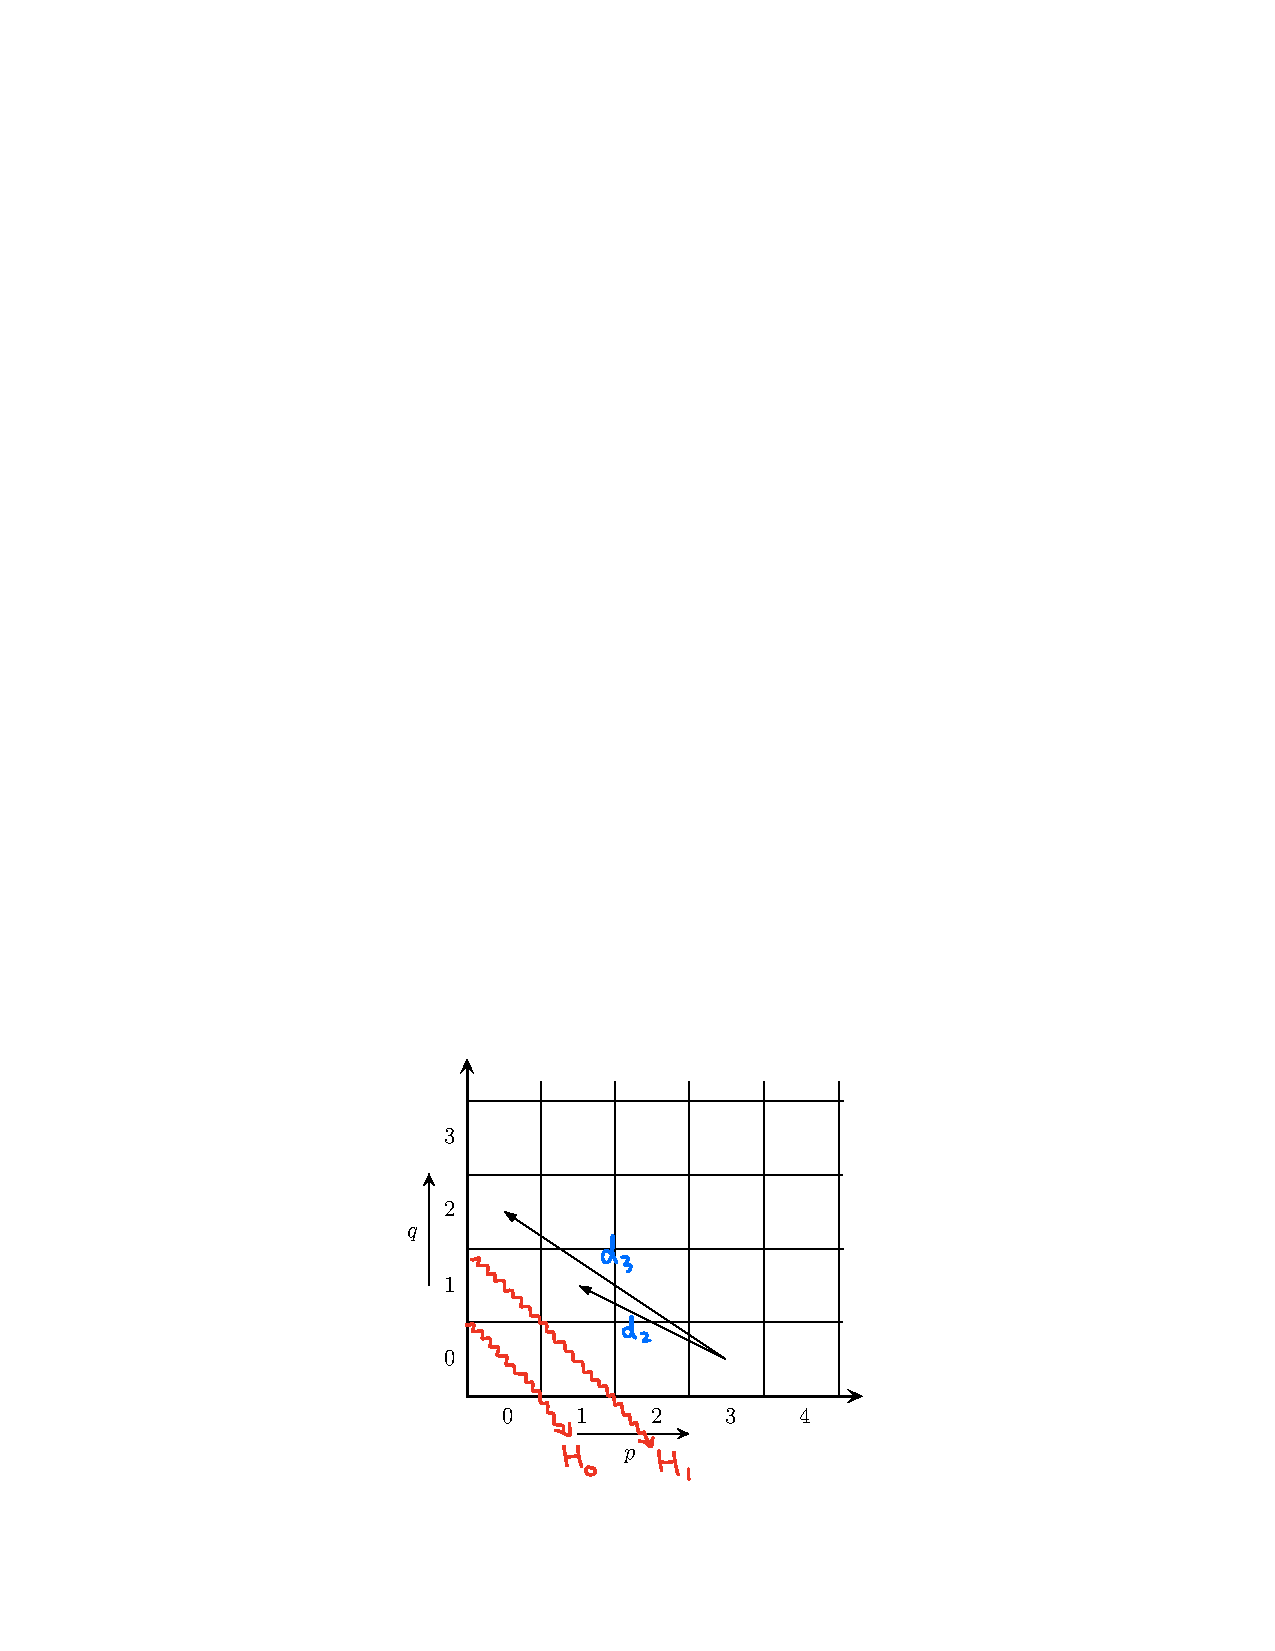
\includegraphics{img/fig1.pdf}
	\caption{spectral sequence differential}
	\label{fig:1}
\end{figure}

\section{User's guide}
\label{sec:examples}
In this section, we will disscuse some examples of spectral sequences mentioned in the last section. These examples are elementary and not computationally involved, yet they clearly demonstrate the power of using spectral sequences as a black box. This section will also use diagrams as much as possible, since they are often the key step in carrying out computations with spectral sequences.\footnote{Due to time constraints, most of the figures are hand-drawn.}
\subsection{(co)homology serre spectral sequence}
In the course, we learned that if $S^l\to S^m\to S^n$ is a fibration then it must be $S^{n-1}\to S^{2n-1}\to S^n$ and $n=1,2,4,8$. The second half of this proposition is known as {\itshape Hopf invariant one problem}, to prove this, we need to use the {\itshape Adams spectral sequence}, which is beyond the scope of this report. Interested readers may consult \cite[Theorem 9.38]{mccleary2001user} as well as Adams’s original paper \cite{adams1, adams2}. A simplified proof can be found in \cite{wang1967cohomology} and a proof based on $K$-theory can be found in \cite{adams1966k}. However, the first half can be proved using the Serre spectral sequence, and we will focus on it.

\begin{theorem}
A necessary (but not sufficient) condition for $S^l\to S^m\to S^n$ to be a fibration is that $l=n-1$ and $m=2n-1$.
\end{theorem}
\begin{proof}
Assuming $S^l\to S^m\to S^n$ is a fibration, then we have the related serre spectral sequence,
\[
E^2_{p,q}=H_p(S^n;H_q(S^l;\mathbb{Z}))\Rightarrow H_{p+q}(S^m;\mathbb{Z})
\]
Using the fact $H_p(S^n;\mathbb{Z})=\mathbb{Z}(\delta_{p,0}+\delta_{p,n})$, so we have:
\[
E^2_{p,q}=\begin{cases}
	\mathbb{Z},&p=0,n \text{~and~} q=0,l\\
	0,&\text{otherwise}
\end{cases}
\]
and $E^2$ looks like Figure~\ref{fig:2}. 
\begin{figure}
	\centering
	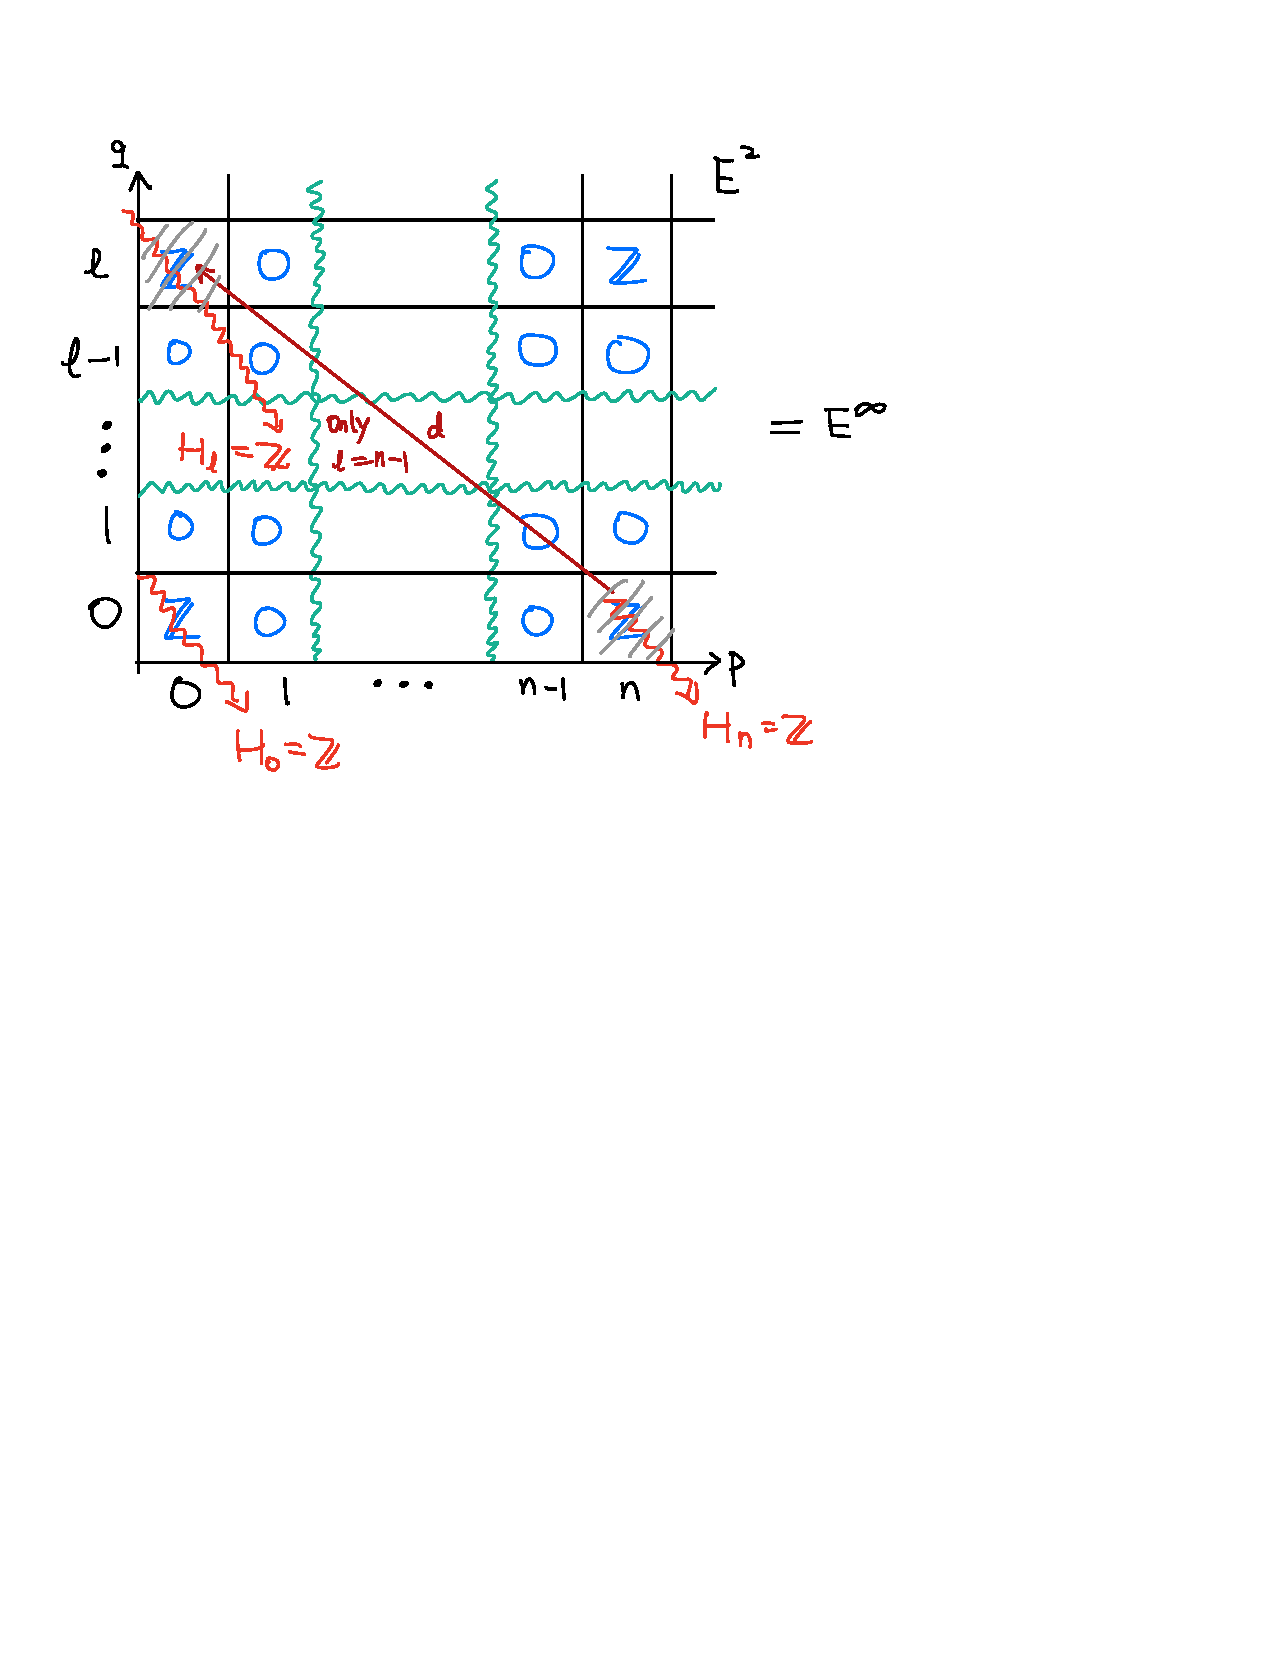
\includegraphics[width=0.7\linewidth]{img/fig2.pdf}
	\caption{Comparing with $H_p(S^m)$, the two shadowed $\mathbb{Z}$ should be killed.}
	\label{fig:2}
\end{figure}
If $l\neq n-1$, every differential is trivial, so $E^2=E^\infty$. In this case, since almost all elements vanish, the extension problems are trivial. We have,
\[
H_0(S^m)=H_{n+l}(S^m)=H_l(S^m)=H_n(S^m)=\mathbb{Z} 
\]
Since we know that $H_p(S^m)=0$ for $p\neq 0,m$, $\mathbb{Z}$ in $(0,l)$ must be {\itshape killed} by $\mathbb{Z}$ in $(n,0)$ using the differential $d_n:\mathbb{Z}\xrightarrow{\mathrm{id}}\mathbb{Z}$, therefore $l$ must equal to $n-1$. Similarly, $n+l$ should equal to $m$.
\end{proof}

From this example, we see that in working with a spectral sequence one can often extract substantial information—sometimes even determine the answer completely—without knowing the explicit form of the differentials $d_r$. This can feel almost “magical”. In fact, much as in the Mayer–Vietoris sequence, the differentials are typically hard to analyze directly. In the examples that follow, we will repeatedly illustrate how far one can go by treating the spectral sequence as a black box in this sense.

The second example concerns the (co)homology groups of the lens space $L(n,q):=S^{2n-1}/\mathbb{Z}_q$. One can compute its homology groups using cellular decompositions. However, the cohomology groups are easier to compute in spectral sequence sense, since cohomology has additional algebraic structure that we can use. We need the following lemma.

\begin{lemma}\label{lemma:2.2}
	The low-degree (co)homology group of the lens space is given by
	\[
	H_2(S^{2n-1}/\mathbb{Z}_k)=0,\quad
	\pi_1(S^{2n-1}/\mathbb{Z}_k)=\mathbb{Z}_k\cong H_1(S^{2n-1}/\mathbb{Z}_k)\cong H^2(S^{2n-1}/\mathbb{Z}_k)
	\]
\end{lemma}
\begin{proof}
	We postpone the explanation of the first equation to the next example, for now, let us focus on the second equation. The first equality comes from the fact that the following fibration (covering map),
	\[
	\mathbb{Z}_k\longrightarrow S^{2n-1}\to S^{2n-1}/\mathbb{Z}_k
	\]
	induces a long exact sequence of homotopy groups. By homotopy group of the sphere, we have the following short exact sequence,\footnote{Maybe you think $\pi_0$ is just a set by definition, so our proof breaks down. However, one can check this fact by using that $S^{2n-1}$ is the universal covering space of $S^{2n-1}/\mathbb{Z}_k$ with Deck group $\mathbb{Z}_k$. Recall that for a universal covering, $\pi_1(S^{2n-1}/\mathbb{Z}_k)$ is isomorphic to the Deck group.}
	\[
	0\to\pi_1(S^{2n-1}/\mathbb{Z}_k)\xrightarrow{\partial}\pi_0(\mathbb{Z}_k)\cong\mathbb{Z}_k\to 0
	\]
	The second equality follows from the Hurewicz theorem. The last equality is then immediate from the universal coefficient theorem, using $H_2(S^{2n-1}/\mathbb{Z}_k)=0$.
\end{proof}
\begin{example}
	The cohomology groups of the lens space are
	\begin{equation}
		H^i({S^{2n-1}/\mathbb{Z}^k})=\begin{cases}
			\mathbb Z, & i=0,\ 2n-1,\\
			\mathbb Z_k, & i\ \text{even and } 2\le i\le 2n-2,\\
			0, & \text{otherwise}.
		\end{cases}
	\end{equation}
	and the cohomology ring is
	\begin{equation}
		\label{lens ring}
		H^\bullet(S^{2n-1}/\mathbb{Z}^k)=\mathbb Z[x,z]/{(kx,\ x^n,\ xz,\ z^2)},
		\qquad |x|=2,\ |z|=2n-1.
	\end{equation}
\end{example}
\begin{proof}
Consider the following fibration:\footnote{Sorry, I cannot explain this fibration well. So let's assume we have a good mathematician friend who tells us this.}
\[
S^1\to S^{2n-1}/\mathbb{Z}_k\to S^{2n-1}/S^1\cong \mathbb{C}P^{n-1}
\]
First, we can show $H_2(S^{2n-1}/\mathbb{Z}_k)=0$ by the homology Serre spectral sequence
\[
E^2_{p,q}=H_p(\mathbb{C}P^{n-1},H_q(S^1))\Rightarrow H_{p+q}(S^{2n-1}/\mathbb{Z}_k)
\]
Here we only need the corner of the $E^2$-page with $p,q\le 2$, which is depicted in Figure~\ref{fig:8}.
\begin{figure}
	\centering
	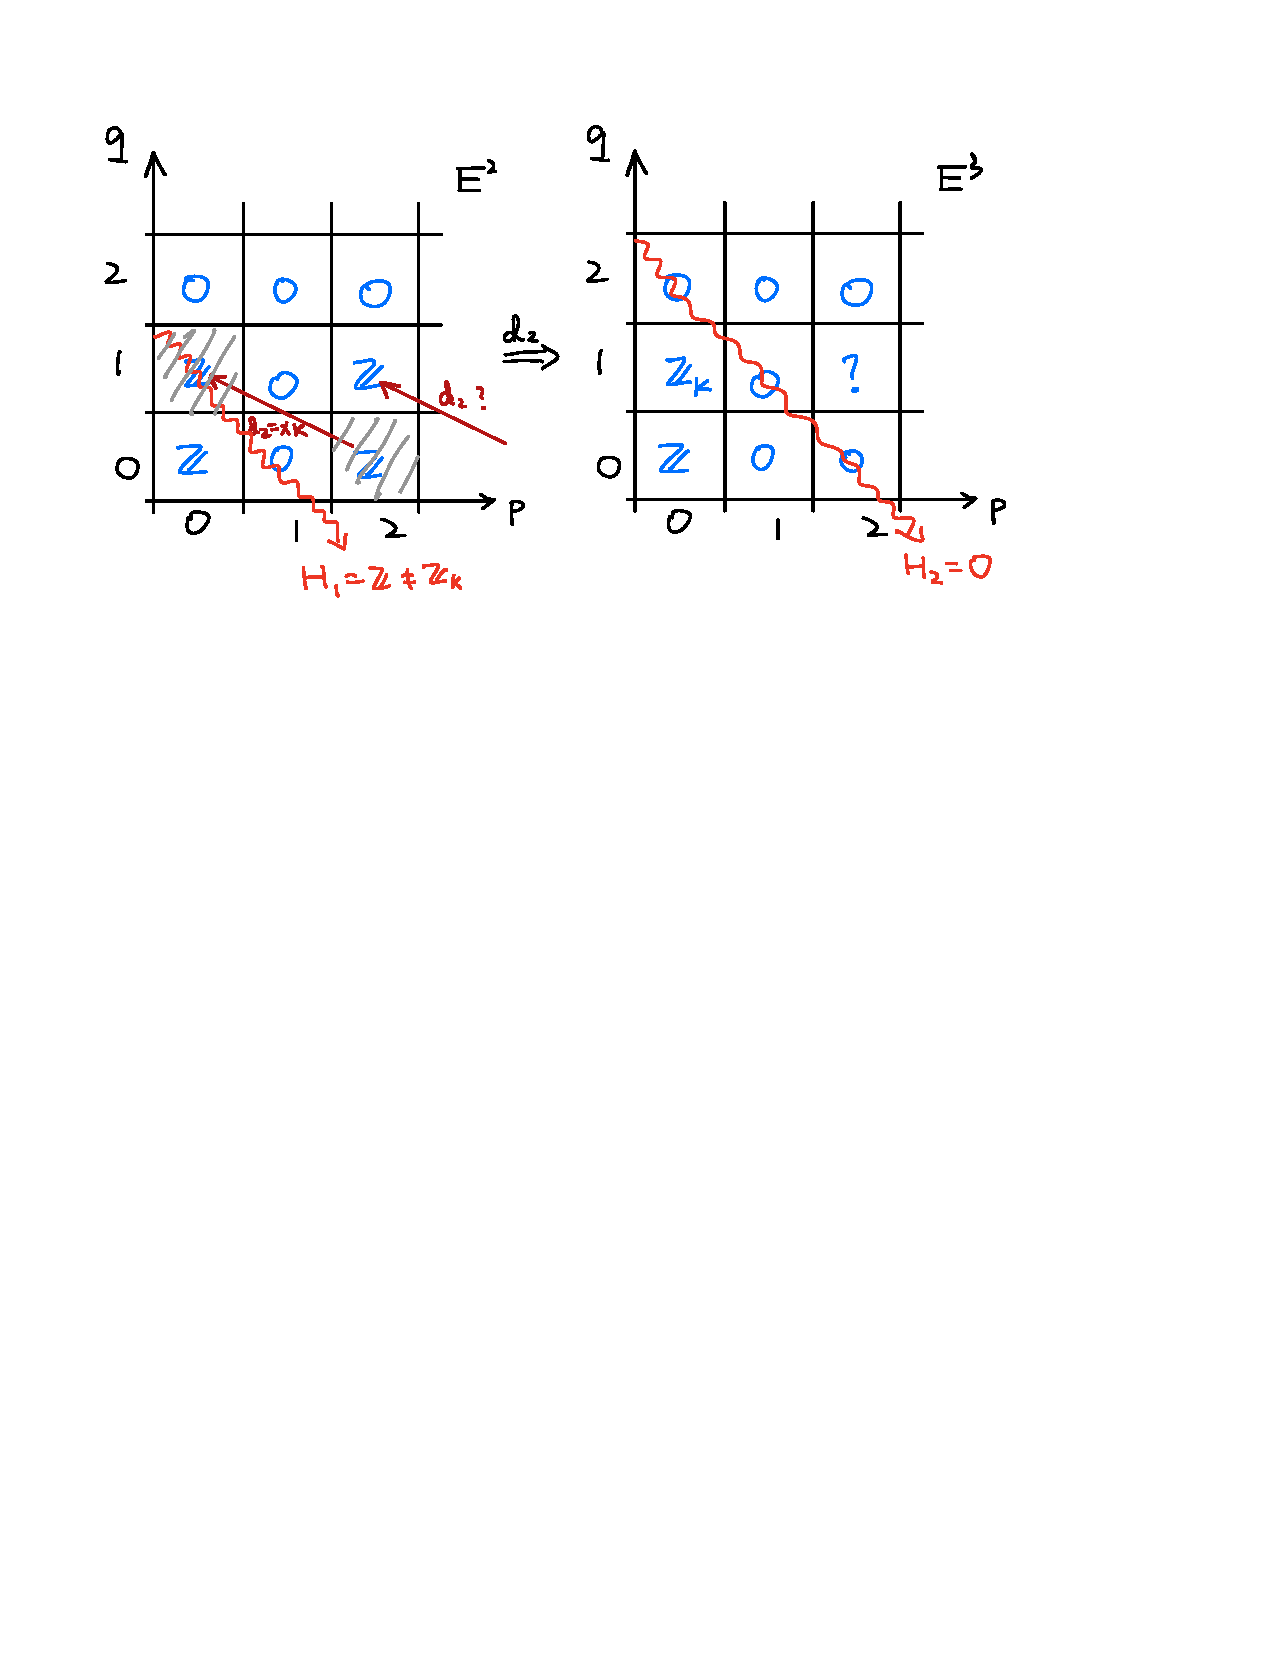
\includegraphics[width=0.8\linewidth]{img/fig4.pdf}
	\caption{We cannot fully describe the $E^\infty$-page, but the $E^3$-page is enough to determine $H_2$.}
	\label{fig:8}
\end{figure}
Since $H_1(S^{2n-1}/\mathbb{Z}_k)\cong\mathbb{Z}_k$\footnote{Note that in the previous lemma \ref{lemma:2.2} we used the assumption $H_2(S^{2n-1}/\mathbb{Z}_k)=0$ only when identifying $H_1(S^{2n-1}/\mathbb{Z}_k)\cong H^2(S^{2n-1}/\mathbb{Z}_k)$, so there is no circular reasoning here.}, the differential $d_2:E^2_{2,0}\to E^2_{0,1}$ must be $\mathbb{Z}\xrightarrow{\times k}\mathbb{Z}$. Hence $E^2_{2,0}$ is killed, and this already suffices to conclude that $H_2(S^{2n-1}/\mathbb{Z}_k)$ vanishes.

Now we turn to the cohomology Serre spectral sequence:
\[
E_2^{p,q}=H^p(\mathbb{C}P^{n-1},H^q(S^1))=H^p(S^1)\otimes H^p(\mathbb{C}P^{n-1}) \Rightarrow H^{p+q}(S^{2n-1}/\mathbb{Z}_k),
\]
which looks like Figure~\ref{fig:9}. 
\begin{figure}
	\centering
	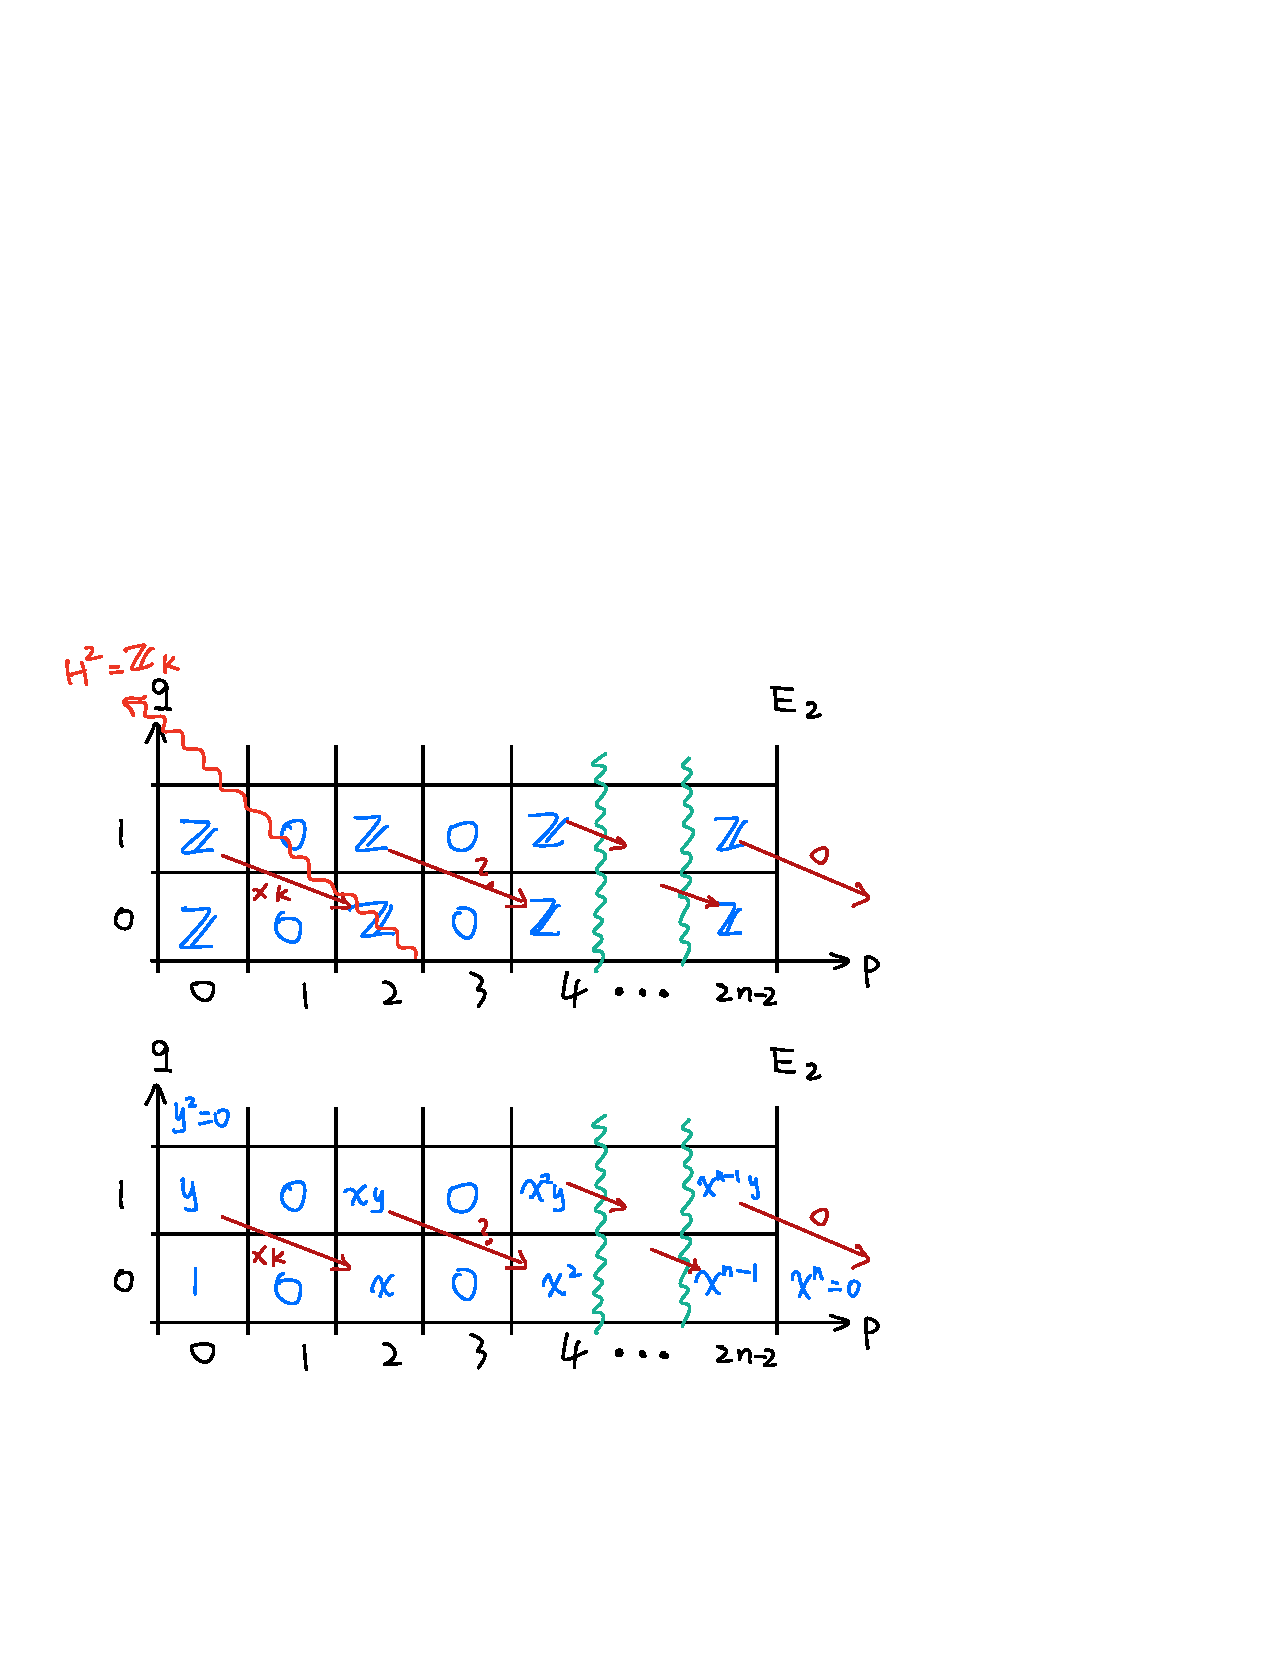
\includegraphics[width=0.8\linewidth]{img/fig5.pdf}
	\caption{$E_2$-page of the cohomology Serre spectral sequence for the lens space}
	\label{fig:9}
\end{figure}
As in our earlier argument for the homology Serre spectral sequence, since
$H^2(S^{2n-1}/\mathbb{Z}_k)\cong\mathbb{Z}_k$, we immediately know that
$d_2:E_2^{0,1}\to E_2^{2,0}$ must be $\mathbb{Z}\xrightarrow{\times k}\mathbb{Z}$.
We cannot make the same conclusion for the other $d_2$'s a priori. However, using
the algebra structure on $E_2$, 
\[
\mathbb{Z}[x]/(x^n)\otimes\Lambda(y)\cong\mathbb{Z}[x,y]/(x^n,y^2),\quad |x|=2,|y|=1
\]
write the generators as $x\in E_2^{2,0}$ and
$y\in E_2^{0,1}$. Since $d_2(y)=ky$ and $d_2(x)=0$, the Leibniz rule \cref{leib} gives
\[
d_2(xy)=d_2(x)\smile y + x\smile d_2(y)=kxy.
\]
Thus $d_2:E_2^{2,1}\to E_2^{4,0}$ is also necessarily
$\mathbb{Z}\xrightarrow{\times k}\mathbb{Z}$, and the same holds for the other
$d_2$ differentials. The $E_3$-page is drawn in Figure~\ref{fig:10}.
\begin{figure}
	\centering
	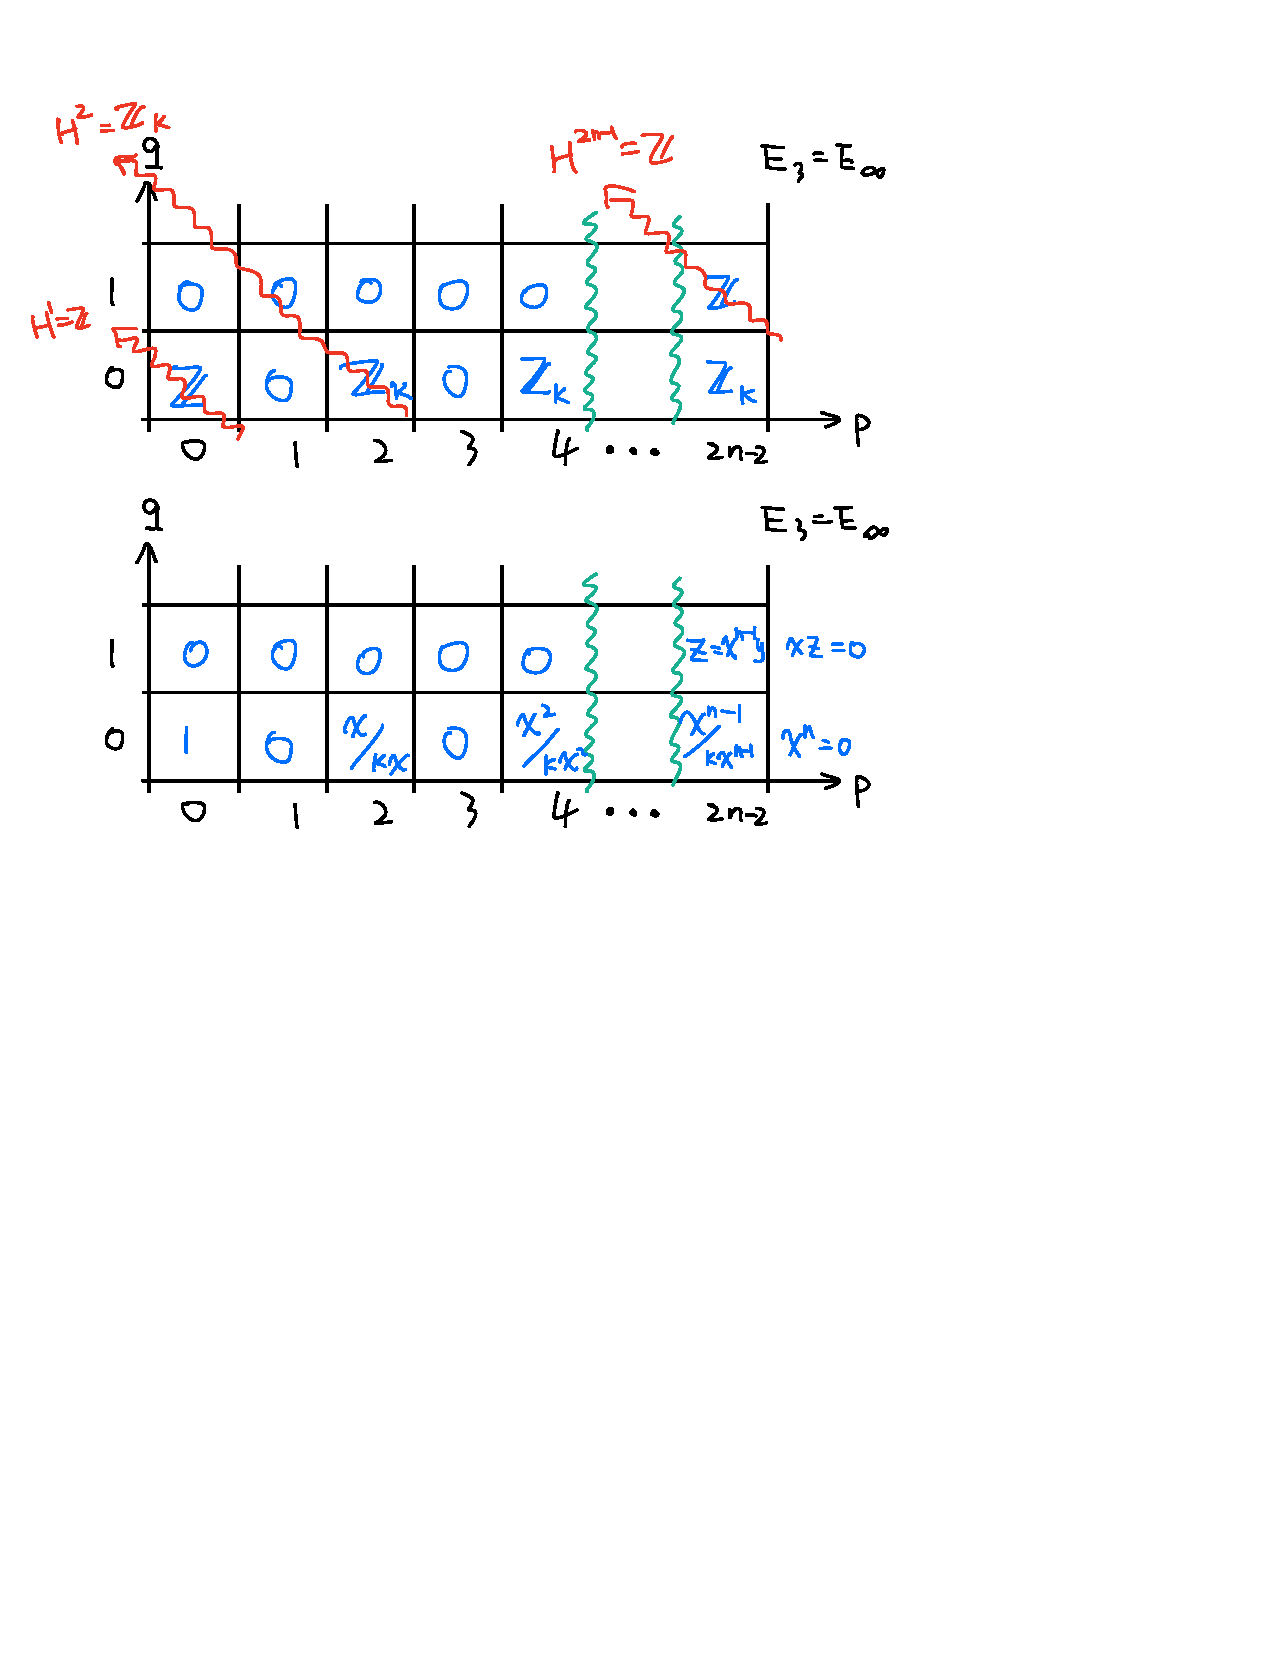
\includegraphics[width=0.8\linewidth]{img/fig6.pdf}
	\caption{$E_3$-page of cohomology Serre spectral sequence for lens space}
	\label{fig:10}
\end{figure}
It is easy to
see that the spectral sequence collapses, so $E_3=E_\infty$. However, note that
the $\mathbb{Z}$ at $E_2^{2n-2,1}$ is not killed. The extension problems are trivial. Returning to the notation in \eqref{lens ring}, it suffices to set $z=x^{n-1}y$. So we complete the proof.
\end{proof}
\begin{remark}
	For the infinite-dimensional lens space, i.e. $S^\infty/\mathbb{Z}_k$, the picture of the spectral sequence makes it clear that the $\mathbb{Z}$ at $E_2^{2n-2,1}$ that is not killed is pushed off to infinity. In effect, one may treat it as if it were killed as well. Therefore the resulting cohomology groups are
	\[
	H^i(S^\infty/\mathbb{Z}_k;\mathbb{Z})\cong
	\begin{cases}
		\mathbb{Z}, & i=0,\\
		\mathbb{Z}_k, & i\ \text{even and } i>0,\\
		0, & i\ \text{odd}.
	\end{cases}
	\]
\end{remark}
To obtain the homology groups and (co)homology groups with different coefficients, one can use the {\itshape universal coefficient theorem}, the answer is:
$$
	H_i\left(S^{2n-1}/\mathbb{Z}_k;\mathbb Z\right)\cong
	\begin{cases}
		\mathbb Z, & i=0,\ 2n-1,\\
		\mathbb Z_k, & i\ \text{odd and } 1\le i\le 2n-3,\\
		0, & \text{otherwise},
	\end{cases}
$$
$$
H_i\left(S^{2n-1}/\mathbb{Z}_k;\mathbb R\right)\cong
\begin{cases}
	\mathbb R, & i=0,\ 2n-1,\\
	0, & \text{otherwise},
\end{cases}
\quad
H^i\!\left(S^{2n-1}/\mathbb{Z}_k;\mathbb R\right)\cong
\begin{cases}
\mathbb R, & i=0,\ 2n-1,\\
0, & \text{otherwise}.
\end{cases}
$$
\[
H_i\!\left(S^{2n-1}/\mathbb{Z}_k;\mathbb Z_q\right)\cong
\begin{cases}
	\mathbb Z_q, & i=0,\ 2n-1,\\
	\mathbb Z_{\gcd(k,q)}, & 1\le i\le 2n-2,\\
	0, & \text{otherwise},
\end{cases}
\]
\[
H^i\!\left(S^{2n-1}/\mathbb{Z}_k;\mathbb Z_q\right)\cong
\begin{cases}
	\mathbb Z_q, & i=0,\ 2n-1,\\
	\mathbb Z_{\gcd(k,q)}, & 1\le i\le 2n-2,\\
	0, & \text{otherwise}.
\end{cases}
\]
In the example above, we computed cohomology rather than homology because working in cohomology allows us to bypass a direct analysis of the fibration: the ring structure can be used to constrain, and often determine, the differentials. In fact, for a general {\itshape homology sphere} there is a following consequence from the spectral sequence.
\begin{theorem}[homology Gysin sequence, Theorem 9.17 in \cite{davis2001lecture}]\label{thm:2.4}
	Let $R$ be a commutative ring. Suppose $F \hookrightarrow E \xrightarrow{\,f\,} B$ is a fibration,
	and suppose $F$ is an $R$-homology $n$-sphere, i.e.
	\[
	H_i(F;R)\cong
	\begin{cases}
		R & \text{if } i=0 \text{ or } n,\\
		0 & \text{otherwise.}
	\end{cases}
	\]
	Assume that $\pi_1(B)$ acts trivially on $H_n(F;R)$.\footnote{This is a subtle point. If it fails, then in computing the $E^2$-page of the Serre spectral sequence one should interpret it as homology with local coefficients derived from the fibration, see \cite[Chapter 5 and Theorem 9.6]{davis2001lecture} for a discussion. However, in this report the base spaces appearing in our computations are all simply connected, so it suffices to work with ordinary homology with constant coefficients.} Then there exists an exact sequence
	(with $R$-coefficients):
	\[
	\cdots \longrightarrow H_r(E) \xrightarrow{\,f_*\,} H_r(B)
	\longrightarrow H_{r-n-1}(B)
	\longrightarrow H_{r-1}(E) \xrightarrow{\,f_*\,} H_{r-1}(B)
	\longrightarrow \cdots .
	\]
\end{theorem}

\subsection{AH spectral sequence}
The first example concerns $K$-theory. The full definition of $K$-theory can be found in the second part of the course. Here, we only need to know that $K$-theory is a cohomology theory in any integer degree such that $K^n(X) = K^{n+2}(X)$. For a point,we have $K^0(*)=\mathbb{Z}$ and $K^{1}(*)=0$.

\begin{theorem}
	\label{CP}
	The K-cohomology of complex projective space is given by:
	\[
	K^{p}(\mathbb{C}P^{n}) = \begin{cases}
			\mathbb{Z}^{n+1}, &p ~\text{even}\\
			0,&\text{otherwise}
		\end{cases}
	\]
\end{theorem}
\begin{proof}
Consider the following trivial fibration,
\[
*\to\mathbb{C}P^{n}\to\mathbb{C}P^n
\]
from the AH spectral sequence, we have:
\[
E_2^{p,q}=H^p(\mathbb{C}P^n;K^q(*))\Rightarrow K^{p+q}(\mathbb{C}P^n)
\]
using the cohomology group of $\mathbb{C}P^n$ which is given by $H^p(\mathbb{C}P^n;\mathbb{Z})=\mathbb{Z}$ for $0\leq p\leq 2n$, $p$ even, and $0$ otherwise. So the $E_2$-page looks like Figure~\ref{fig:6}.
\begin{figure}
	\centering
	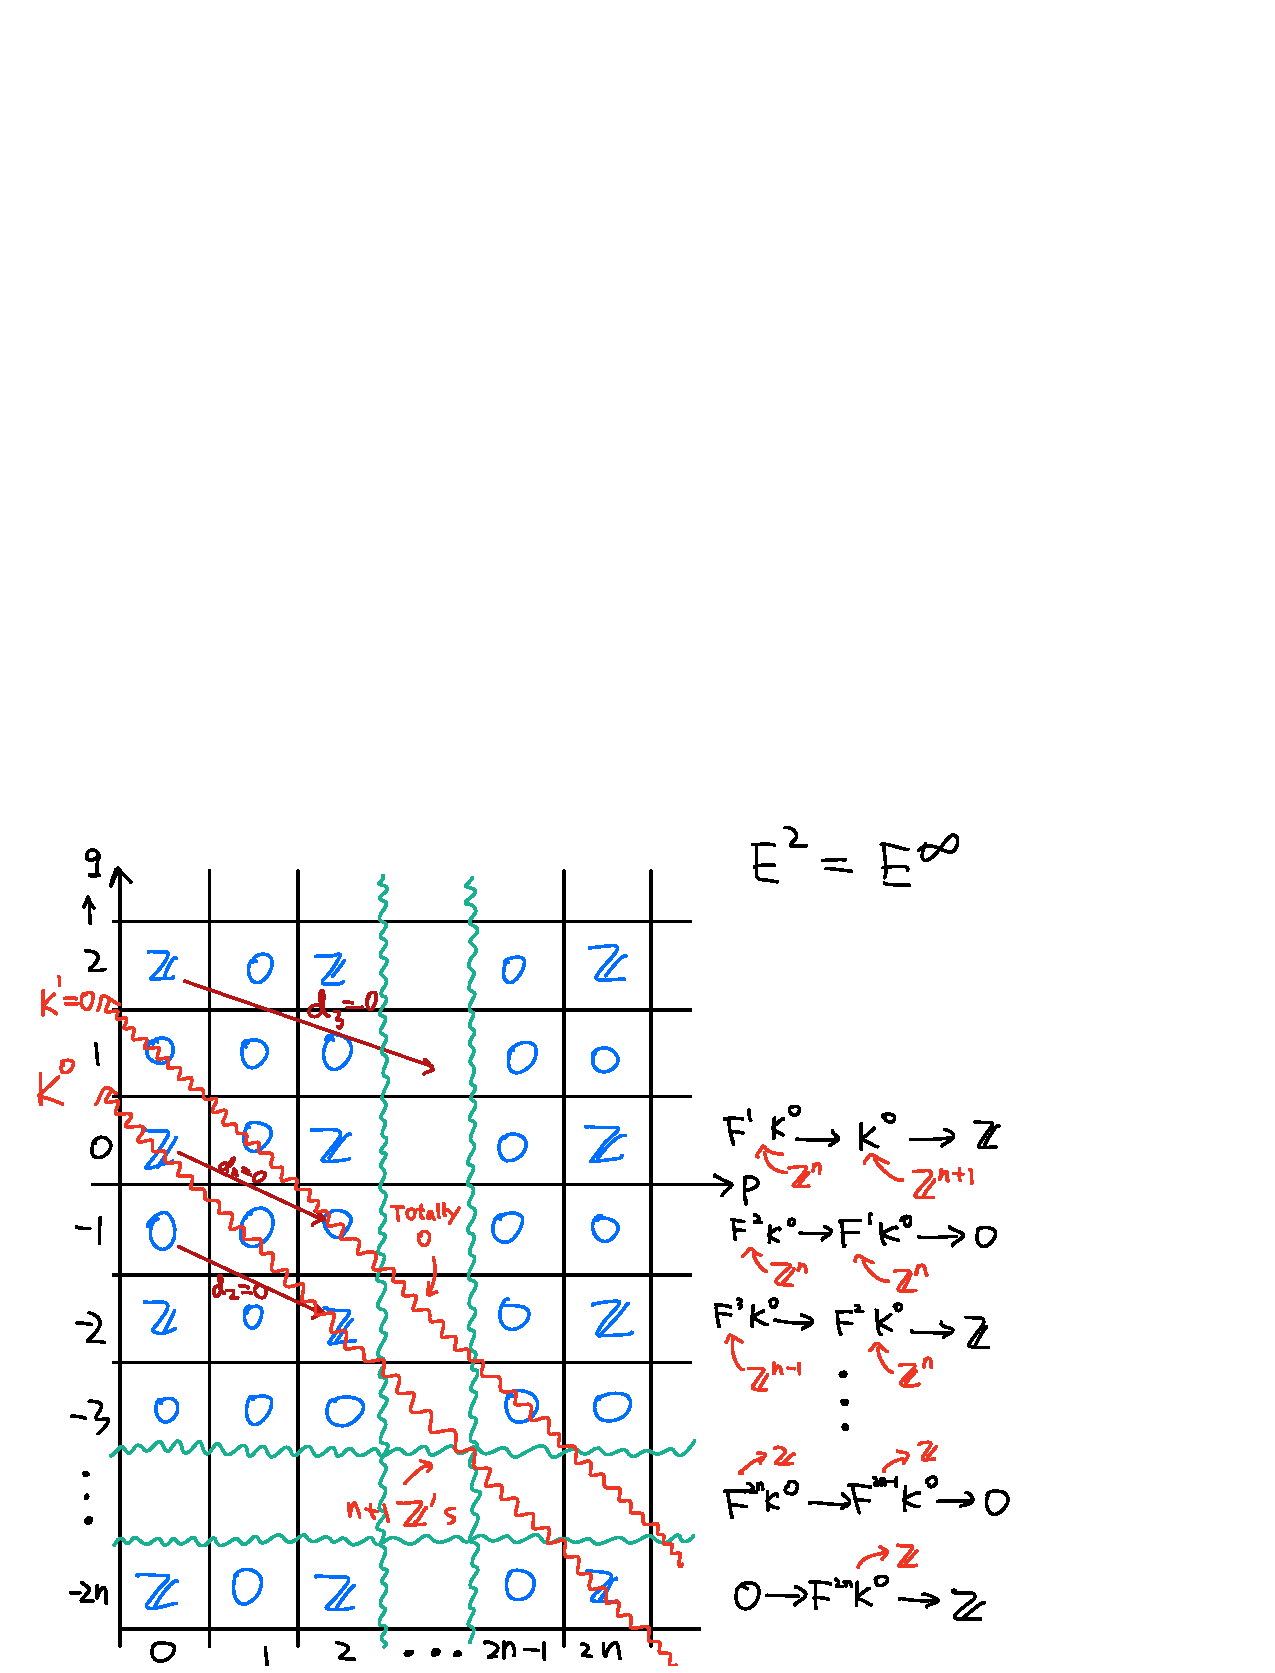
\includegraphics[width=0.8\linewidth]{img/fig3.pdf}
	\caption{We use the fact that $A\to B\to \mathbb{Z}$ implies $B=A\oplus \mathbb{Z}$ to recover $K^0$.}
	\label{fig:6}
\end{figure}
Recall that $K$-theory can be defined for negative integers, so here we have a half-plane rather than first quadrant spectral sequence. Obviously, this spectral sequence collapses at $E_2=E_\infty$. Using the fact that {\itshape if the last term in a short exact sequence of abelian groups is free abelian, then the sequence splits}, we complete the proof.
\end{proof}

The next example concerns the oriented bordism groups in dimensions at most four. Bordism groups can be considered as an additive gneralized homology theory, as we said in remark \ref{LSAH}. The details of its definition can be found in the second half of the course. Here we only need the first few bordism groups of a point.
\begin{lemma}
	\begin{equation}
		\label{bordism}
		\Omega_q^{SO}(*)=\begin{cases}0,&q<0\text{~or~}q=1,2,3,\\\mathbb{Z},&\text{~for~}q=0,4.\end{cases}
	\end{equation}
\end{lemma}
And the bordism groups are defined only for non-negative integers. Before we proceed to the example, we introduce {\itshape edge morphisms} first.

For a fist quadrant homology spectral sequence, it is clear that we have the following monomorphisms and epimorphisms for all $p,q\geq 0$:
\[
\begin{gathered}
	E^{\infty}_{p,0}\hookrightarrow\cdots \hookrightarrow E^{r+1}_{p,0}\hookrightarrow E^{r}_{p,0}\hookrightarrow\cdots\hookrightarrow E^2_{p,0}\\
	E^{\infty}_{0,q}\twoheadleftarrow\cdots \twoheadleftarrow E^{r+1}_{0,q}\twoheadleftarrow E^{r}_{0,q}\twoheadleftarrow\cdots\twoheadleftarrow E^2_{0,q}
\end{gathered}
\]
For a first quadrant spectral sequence, \eqref{extension} give us two morphisms:
\[
\begin{gathered}
F_{p-1}H_p\to H_{p}\to E^\infty_{p,0} \Rightarrow H_p\twoheadrightarrow E^{\infty}_{p,0}\\
0\to F_{0}H_{q}\to E^\infty_{0,q}\Rightarrow E^\infty_{0,q} \cong F_{0}H_{q}\hookrightarrow H_q
\end{gathered}
\]
Then we conclude:
\begin{equation}
	\label{edge}
	E^2_{0,q}\twoheadrightarrow E^{\infty}_{0,q}\hookrightarrow H_q,\quad H_p\twoheadrightarrow E^{\infty}_{p,0}\hookrightarrow E^2_{p,0}
\end{equation}
These morphisms are called {\itshape edge morphisms}. The argument in the cohomological case is completely parallel, one only needs to switch $\hookrightarrow$ with $\twoheadleftarrow$, and replace the lower indices by upper indices, so we will not repeat it here.

Moreover, for a path-connected space $B$ in $F\hookrightarrow E\to B$ and a homology theory $h_\bullet$ there is a surjection:\footnote{For homology with constant coefficients, the existence of this surjection is trivial, and in fact it is an isomorphism. In the case of local coefficients, however, one can only conclude that there is a natural surjection \cite[Proposition 5.14]{davis2001lecture}.}
\[
	h_n(F)\twoheadrightarrow H_0(B;h_n(F))
\]
Together with \eqref{edge}, we conclude that there is a morphism:
\begin{equation}
	\label{edge2}
h_n(F)\twoheadrightarrow H_0(B;h_n(F))\cong E_{0,n}^2\twoheadrightarrow E_{0,n}^\infty\hookrightarrow h_n(E)
\end{equation}
This is just the morphism induced by the inclusion $\iota : F\hookrightarrow E$ by the homology theory $h_\bullet$. Now we prove that, in dimensions at most four, the bordism theory is completely determined by the homology groups.
\begin{theorem}
	For a path-connected space $X$, hence $H_0(X;\mathbb{Z})=\mathbb{Z}$, we have
	\begin{equation}
		\Omega_q^{SO}(X)=\begin{cases}
			H_q(X;\mathbb{Z}),&\text{~for~}q=0,1,2,3,\\\mathbb{Z}\oplus H_4(X;\mathbb{Z}),&\text{~for~}q=4.\end{cases}
	\end{equation}
\end{theorem}
\begin{proof}
	Consider the following trivial fibration:
	\[
	*\overset{\iota}{\hookrightarrow} X\xrightarrow{\operatorname{id}} X
	\]
using \eqref{bordism}, the LSAH spectral sequence,\footnote{In the footnote to \cref{thm:2.4}, we pointed out the subtle issue that local coefficient homology groups enter when the base space is not simply connected. However, since \eqref{edge2} already accounts for homology with local coefficients, the proof here applies to arbitrary topological spaces.}
\[
E^2_{p,q}=H_p(X;\Omega^{SO}_q(*))\Rightarrow\Omega^{SO}_{p+q}(X)
\]
looks like Figure~\ref{fig:7} for $p,q\leq 4$.
\begin{figure}
	\centering
	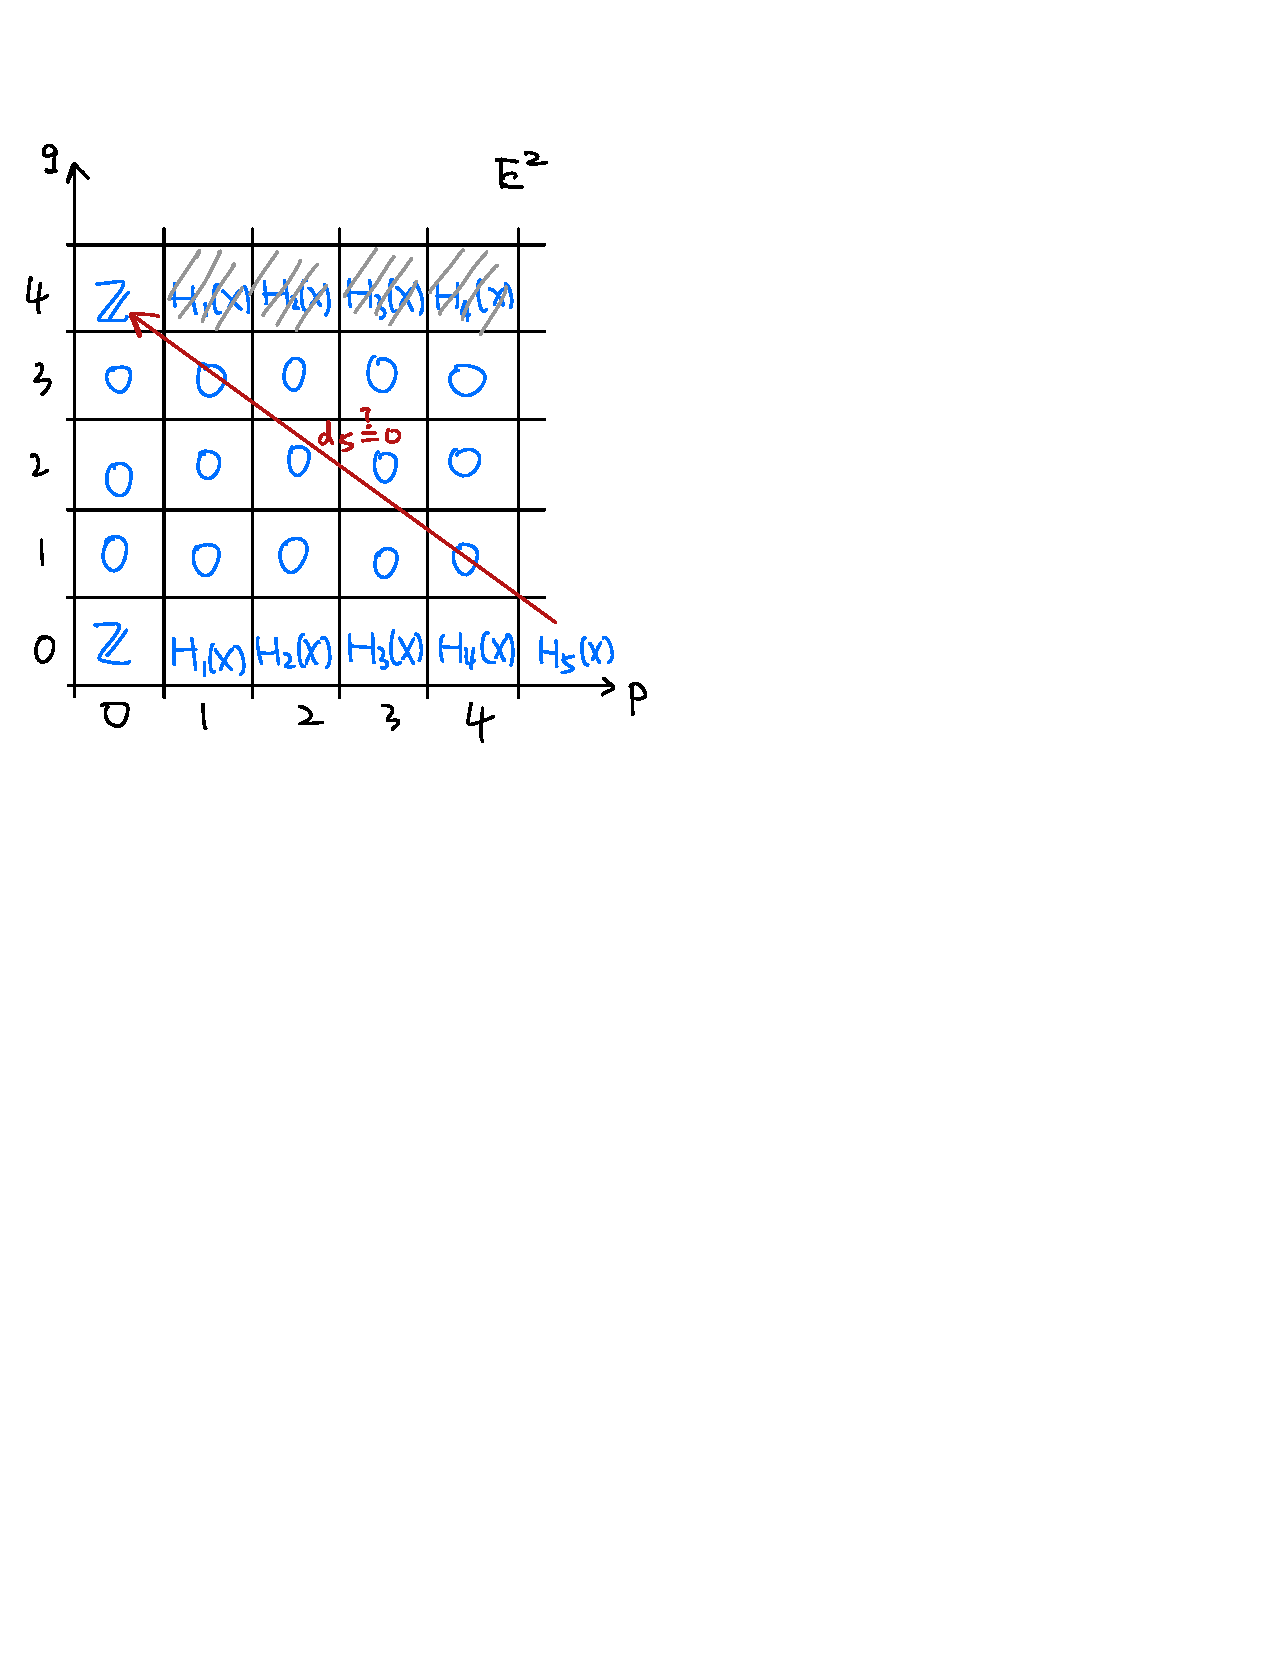
\includegraphics[width=0.45\linewidth]{img/fig8.pdf}
	\caption{The most important differential in our computation is $d_5$, however $E^2_{0,q}=E^\infty_{0,q}$ implies it is trivial. Although the shadowed blocks can not be fully determined in $E^\infty$, it is enough to compute $\Omega_{q\leq 4}^{SO}(X)$.}
	\label{fig:7}
\end{figure}
\eqref{edge2} gives us the following edge morphism:
\[
\Omega^{SO}_q(\iota)=\left(\Omega^{SO}_q(*)\twoheadrightarrow H_0(X;\Omega^{SO}_q(*))\cong E_{0,q}^2\twoheadrightarrow E_{0,q}^\infty\hookrightarrow \Omega^{SO}_q(X)\right)
\]
Note that the constant map $c:X\to *$ satisfies $c\circ\iota=\mathrm{id}_*$. Hence $\Omega_{q}^{SO}(c)\circ \Omega_q^{SO}(\iota)=\Omega_q^{SO}(\mathrm{id}_*)=\mathrm{id}_{\Omega^{SO}_q(*)}$ which implies that $\Omega^{SO}_q(\iota)$ is injective. So we conclude that $E_{0,q}^2=E^{\infty}_{0,q}$, which implies that all differentials arriving or emanating from the vertical axis must be zero. The $E^{\infty}$-page can not be fully determined, but it looks like the right panel of Figure~\ref{fig:7b}. It is enough to compute $\Omega^{SO}_{q\leq 4}(X)$.
\begin{figure}
	\centering
	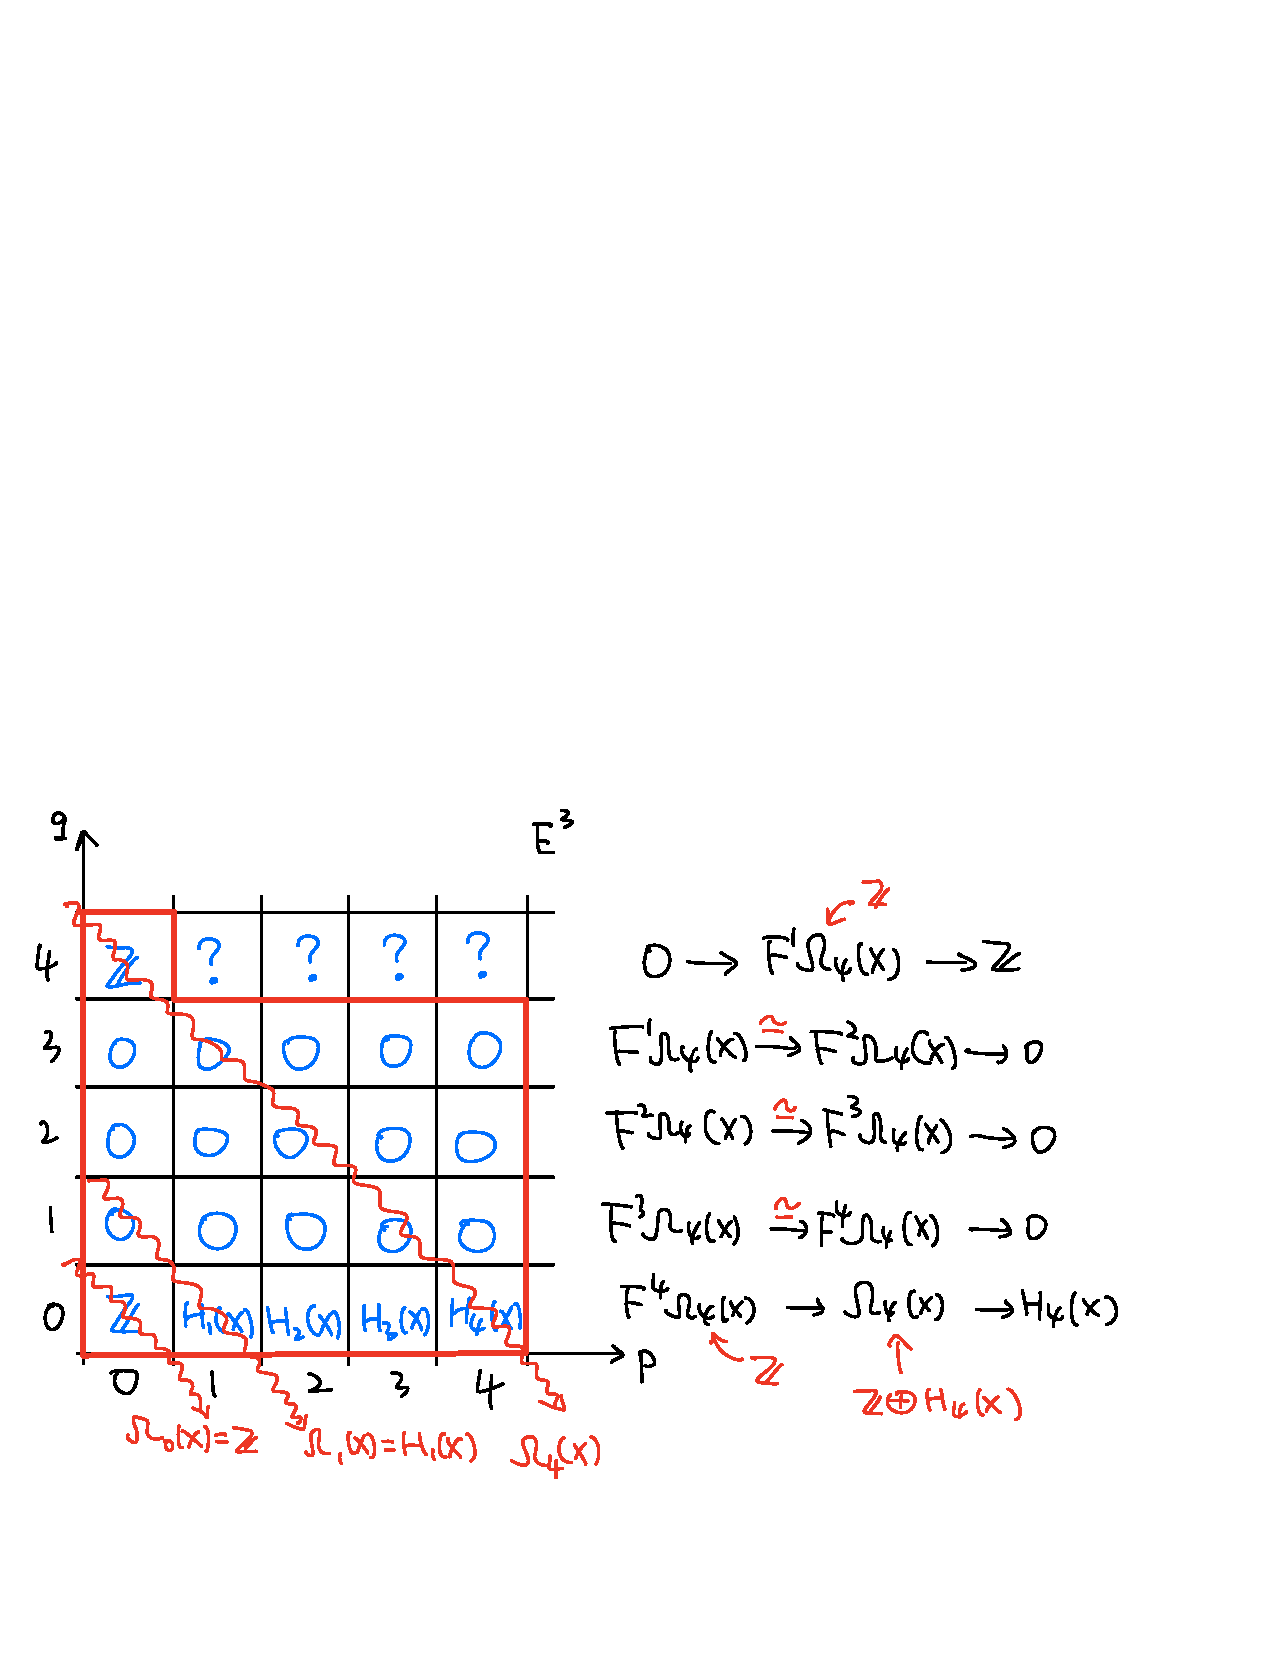
\includegraphics[width=0.8\linewidth]{img/fig7.pdf}
	\caption{$E^3$-page, the part inside the red box is stable.}
	\label{fig:7b}
\end{figure}
\end{proof}
\subsection{(co)homology LHS spectral sequence}
\label{sec:lift}
As the examples in the previous sections show, one can often exploit the full power of a spectral sequence even without knowing the differentials explicitly. The examples in this section take the opposite approach: chosen primarily for pedagogical purposes, they illustrate that in many situations a spectral sequence may only narrow the answer down to a finite range of possibilities rather than determine it uniquely.

In particular, we will focus on the (co)homology of finite groups as defined in the second part of this course. We do not intend to study group (co)homology in any depth, it will serve only as a setting in which to demonstrate spectral sequence computations.

Our first example concerns cyclic groups, before turning to it, we need some knowledge of $C_2\cong \mathbb{Z}_2$,
\begin{lemma}[\S6.2 in \cite{weibel1994introduction}]
	The homology of the cyclic group of order 2 with coefficients $\mathbb{Z}$ or $\mathbb{Z}_2$ is given by,
	\[
	H_p(C_2;\mathbb{Z})=\begin{cases}
		\mathbb{Z},&p=0\\
		\mathbb{Z}_2,&p \text{~odd}\\
		0,&\text{otherwise}
	\end{cases},\quad H_n(C_2;\mathbb{Z}_2)=\mathbb{Z}_2
	\]
	and the integral cohomology ring is given by
	\[
	H^\bullet(C_2;\mathbb{Z})=\mathbb{Z}_2[x],\text{~with~} |x|=1
	\]
	Actually, for any cyclic group, the even dimensional homology groups vanish.
\end{lemma}
\begin{example}
	The homology groups of $C_4$ are given by:
	\[
		H_p(C_4;\mathbb{Z})=\begin{cases}
		\mathbb{Z},&p=0\\
		\mathbb{Z}_4,&p \text{~odd}\\
		0,&\text{otherwise}
		\end{cases}
	\]
\end{example}
\begin{proof}[Partial proof]
	Consider the following group extension,
	\begin{equation}
		\label{cyc}
		C_2\to C_4\to C_2
	\end{equation}
	According to the LHS spectral sequence, we have:
	\[
	E^2_{p,q}=H_p(C_2;H_q(C_2;\mathbb{Z}))\Rightarrow H_{p+q}(C_4;\mathbb{Z})
	\]
	According to the above Lemma, the $E^2$-page can be described by Figure~\ref{fig:3}.
	\begin{figure}
		\centering
		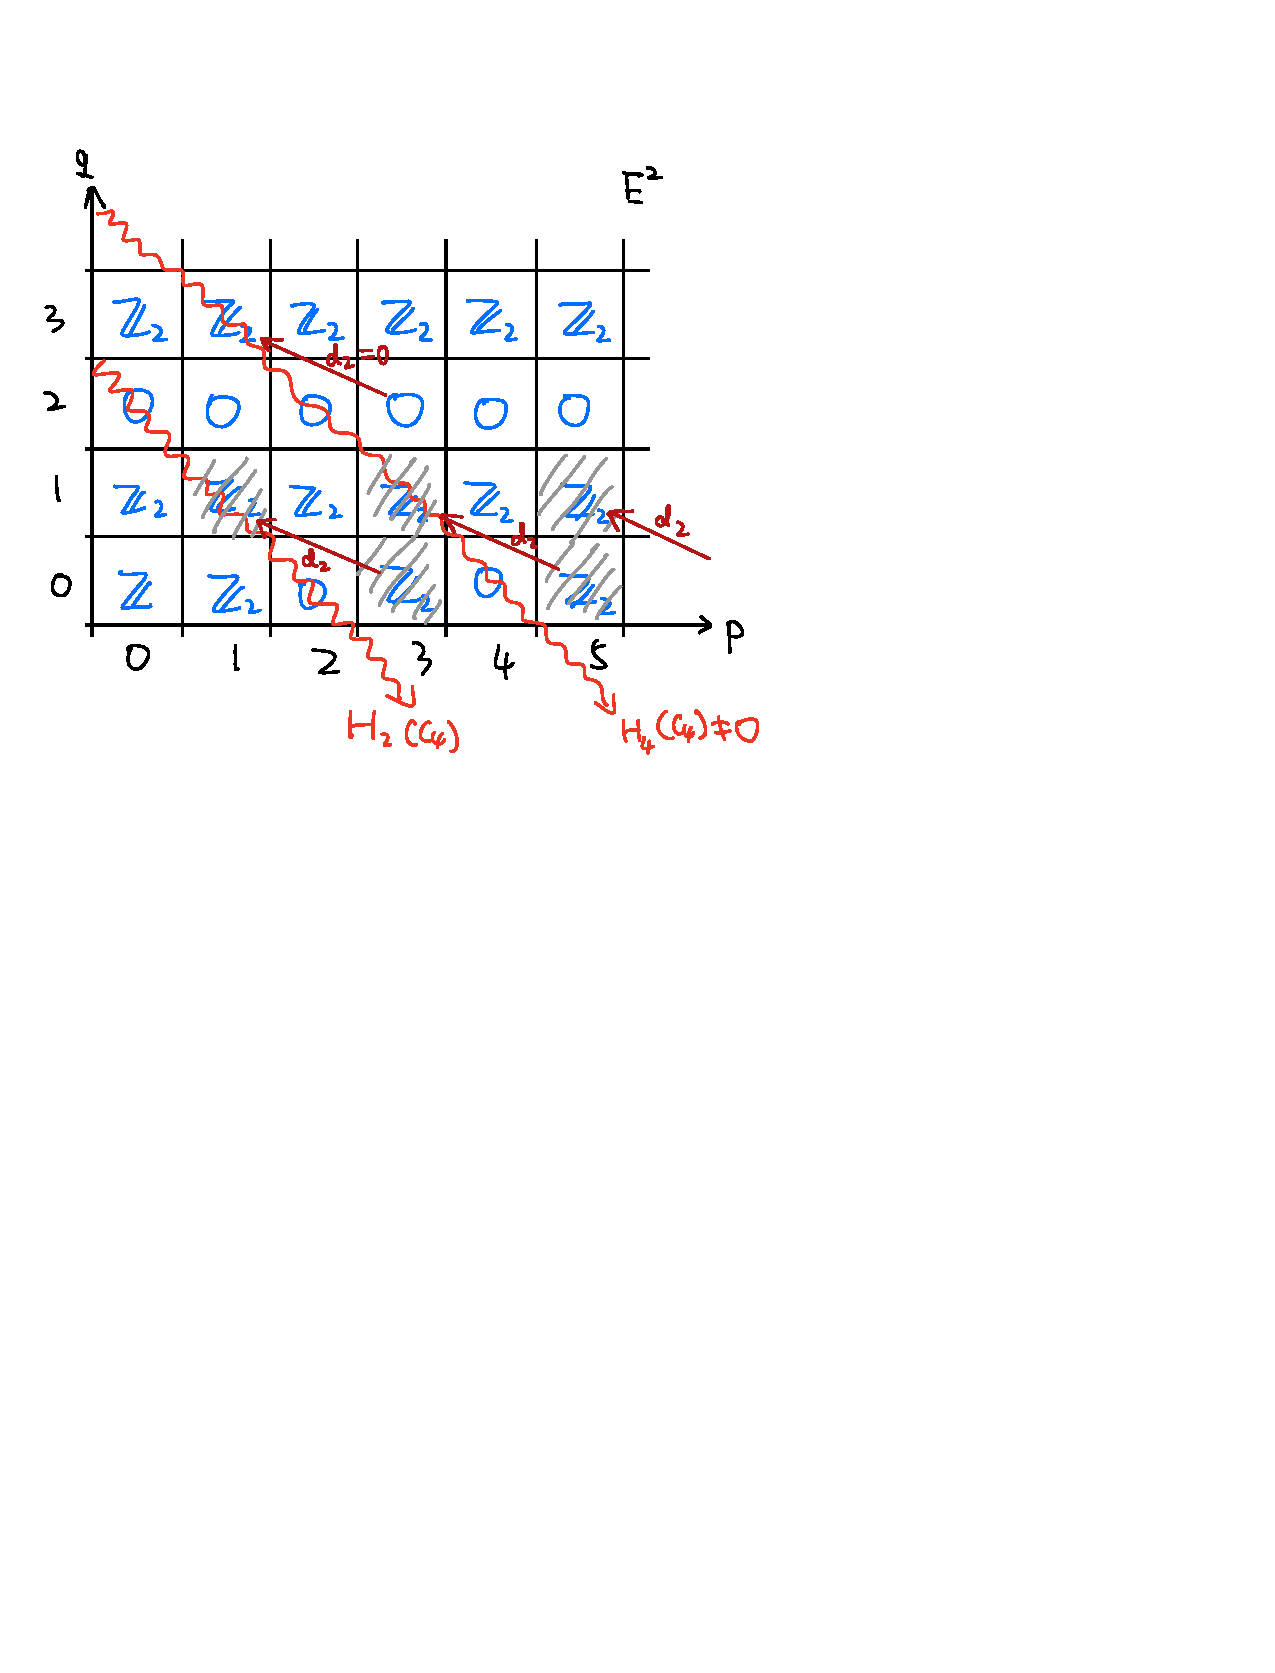
\includegraphics[width=0.7\linewidth]{img/fig9.pdf}
		\caption{The $E^2$-page,  $E^2_{1,1},E^2_{3,1},E^2_{5,1},\cdots$ should be killed, but $d_2$ cannot help us kill $E^2_{1,3},E^2_{3,3},E^2_{5,3},cdots$.}
		\label{fig:3}
	\end{figure}
	We know that $H_n(C_4;\mathbb{Z})=0$ for $n>0$ even. Then the $\mathbb{Z}_2$'s in $E^2_{1,1},E^2_{3,1},E^2_{5,1},\cdots$ must die and their only chance is to be killed by $d_2$ from the $\mathbb{Z}_2$'s in $E^2_{3,0},E^2_{5,0},E^2_{7,0},\cdots$. There are no other possible non-trivial differentials $d_2$ and hence $E^3$ is as in Figure~\ref{fig:3b}.
	
	\begin{figure}
		\centering
		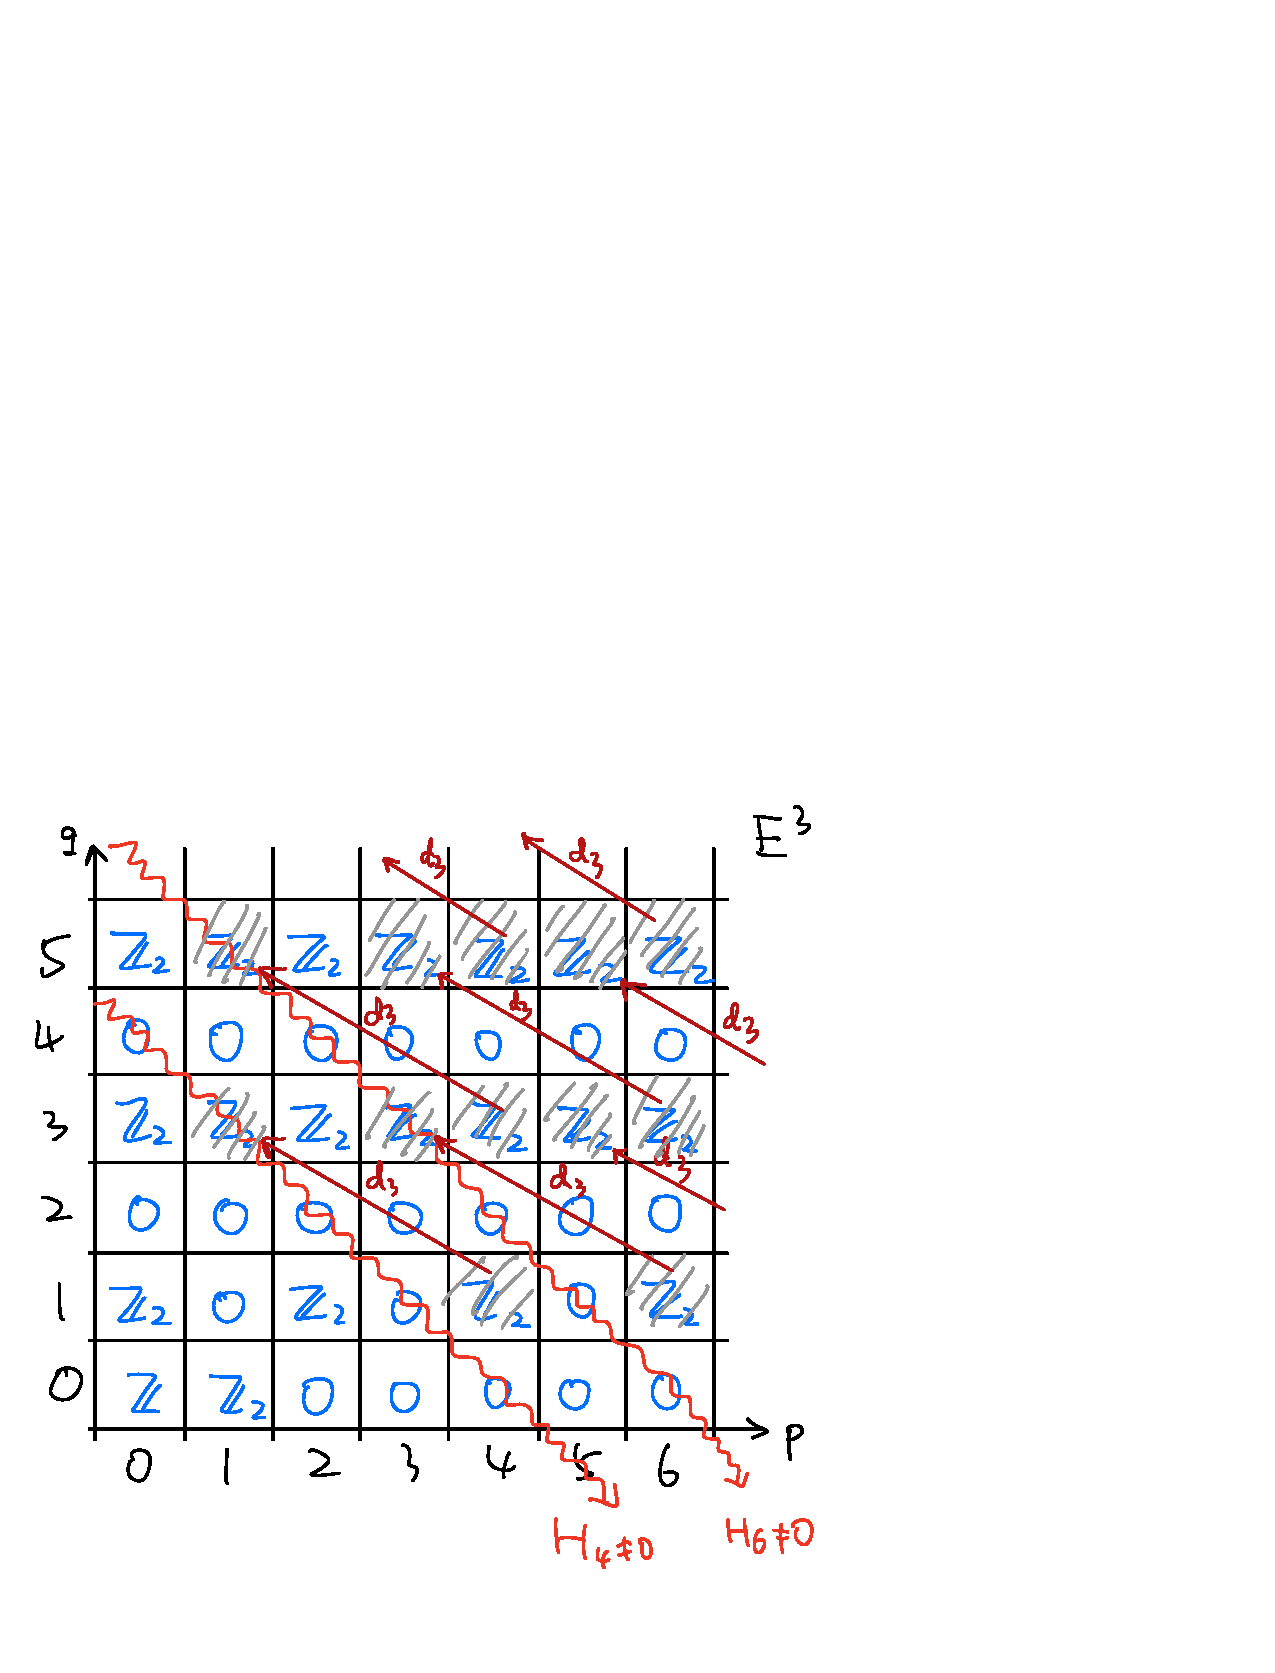
\includegraphics[width=0.6\linewidth]{img/fig10.pdf}
		\caption{The $E^3$-page,  $d_3$ can help us kill $E^{1,3},E^{3,3},E^{5,3},cdots$ as well as other shadowed blocks.}
		\label{fig:3b}
	\end{figure}
	
	Again there are $\mathbb{Z}_2$'s in diagonals contributing to $H_n(C_4;\mathbb{Z})$ with $n>0$ even, hence they should be killed by $d_3$. Then $E^4$ looks like Figure~\ref{fig:4}.
		\begin{figure}
		\centering
		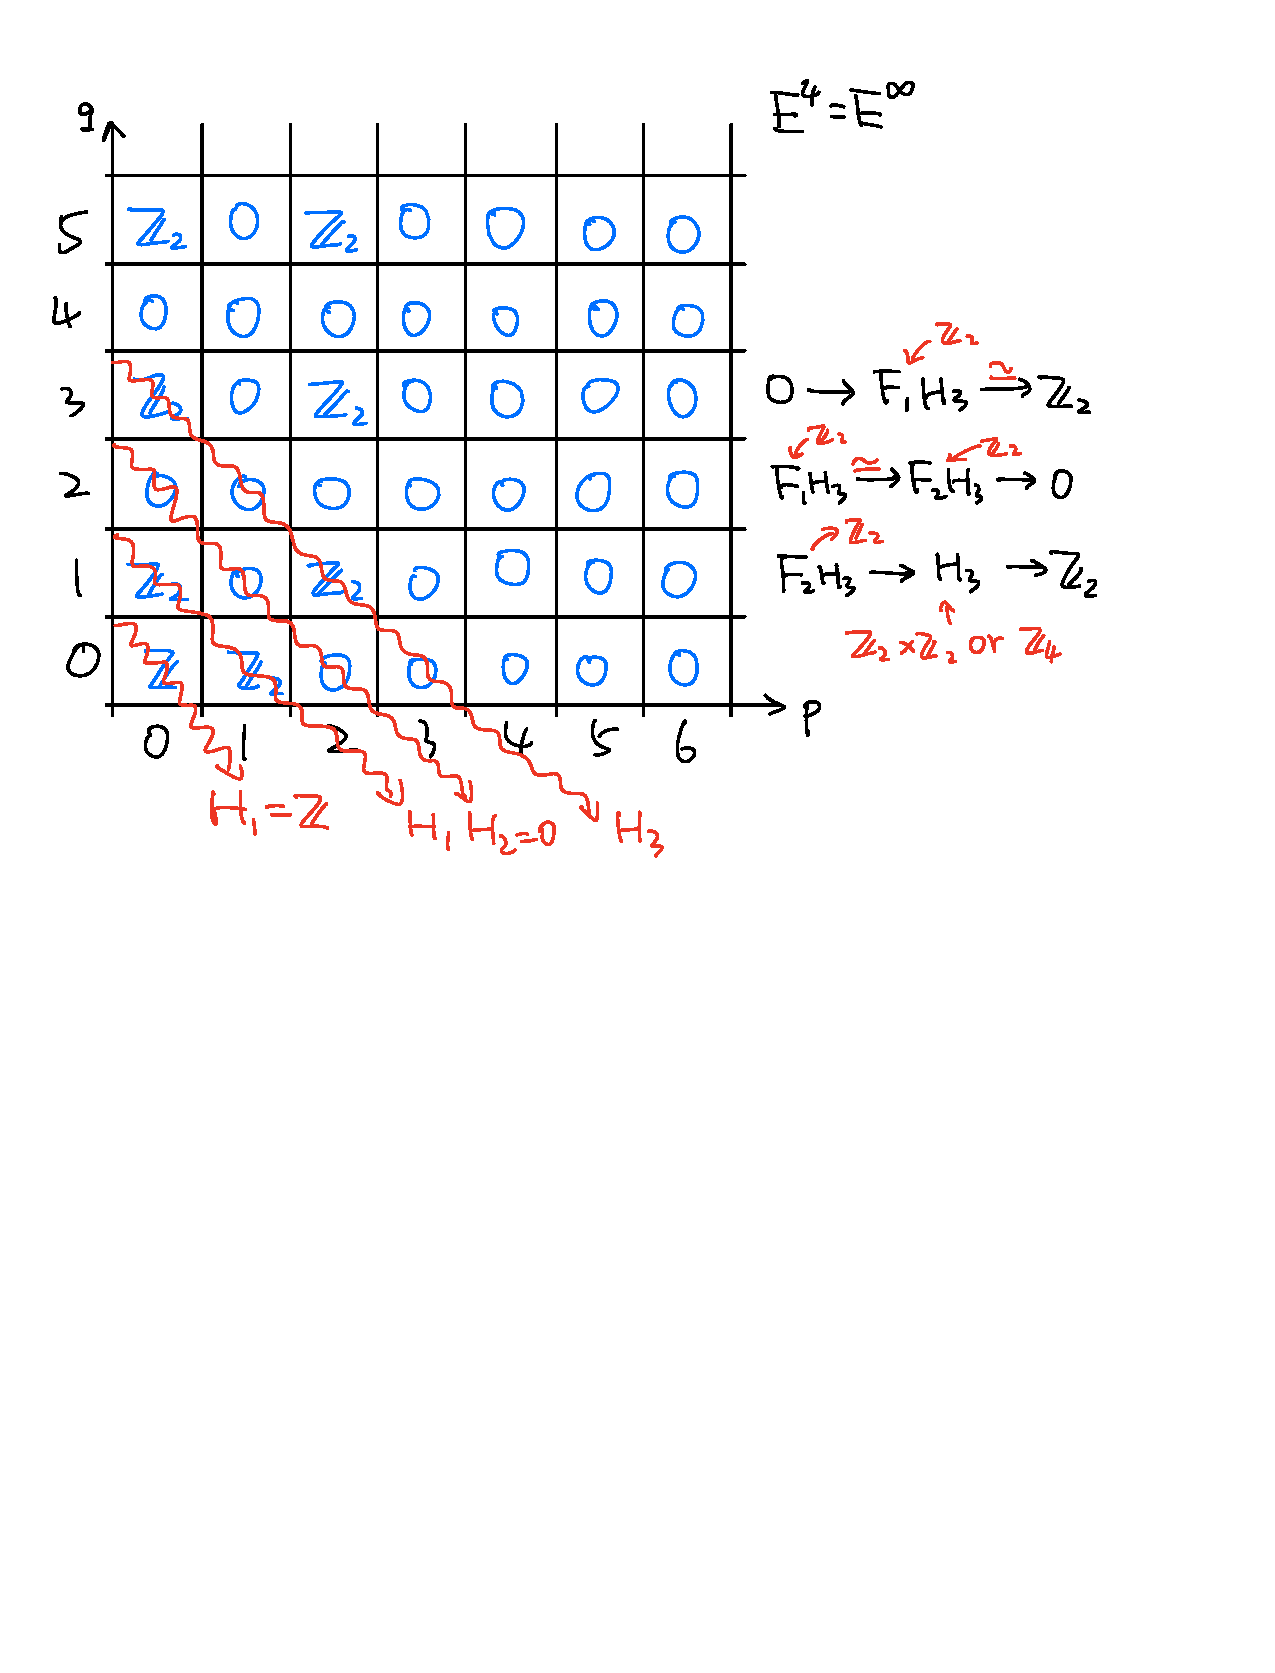
\includegraphics[width=0.8\linewidth]{img/fig11.pdf}
		\caption{$E^4$-page of LHS spectral sequence of $C_2\to C_4\to C_2$}
		\label{fig:4}
	\end{figure}
	It is clear that the spectral sequence {\itshape collapses} at $E^4= E^\infty$. It is easy to show that $H_0(C_4;\mathbb{Z})=\mathbb{Z}$, but for $n$ odd, we encounter the following extension problem:
	\[
	\mathbb{Z}_2\to H_n (C_4;\mathbb{Z}_2)\to \mathbb{Z}_2
	\]
	There are two solutions, either $H_{\text{odd}}(C_4;\mathbb{Z})=\mathbb{Z}_4$ or $H_{\text{odd}}(C_4;\mathbb{Z})=\mathbb{Z}_2\times\mathbb{Z}_2$. The right answer is $\mathbb{Z}_4$, but we need more input to determine this.
\end{proof}
\begin{remark}
	Indeed, the computation of the (co)homology of a cyclic group can be related to our earlier computation for lens spaces via the identification $BC_m \simeq L(\infty,m)$.
\end{remark}
Now, we turn to the cohomology ring.
\begin{example}
	\label{2.12}
	The integral cohomology ring of $C_4$ is given by:
	\[
	H^\bullet(C_4;\mathbb{Z})=\mathbb{Z}[z]/(4z),\text{~with~} |z|=2
	\]
\end{example}
\begin{proof}[Partial proof]
	The group extension given by \cref{cyc} is a central extension, then the LHS spectral sequence is:\footnote{The notation here may be a bit nonstandard from a mathematician’s point of view. One would usually write the polynomial ring as $\mathbb{F}_2[x,y]$. For physicists, however, we will treat this as essentially the same, in the sense that $\mathbb{Z}_2 \cong (-1)^{\mathbb{F}_2}$.
	}
	\begin{equation}
		E_2^{p,q}=H^{p}(C_2;\mathbb{Z})\otimes H^{q}(C_2;\mathbb{Z})\cong\mathbb{Z}[x,y]/(2x,2y)\Rightarrow H^{p+q}(C_4;\mathbb{Z})
	\end{equation}
	The $E_2$-page looks like Figure~\ref{fig:5}.
	\begin{figure}
		\centering
		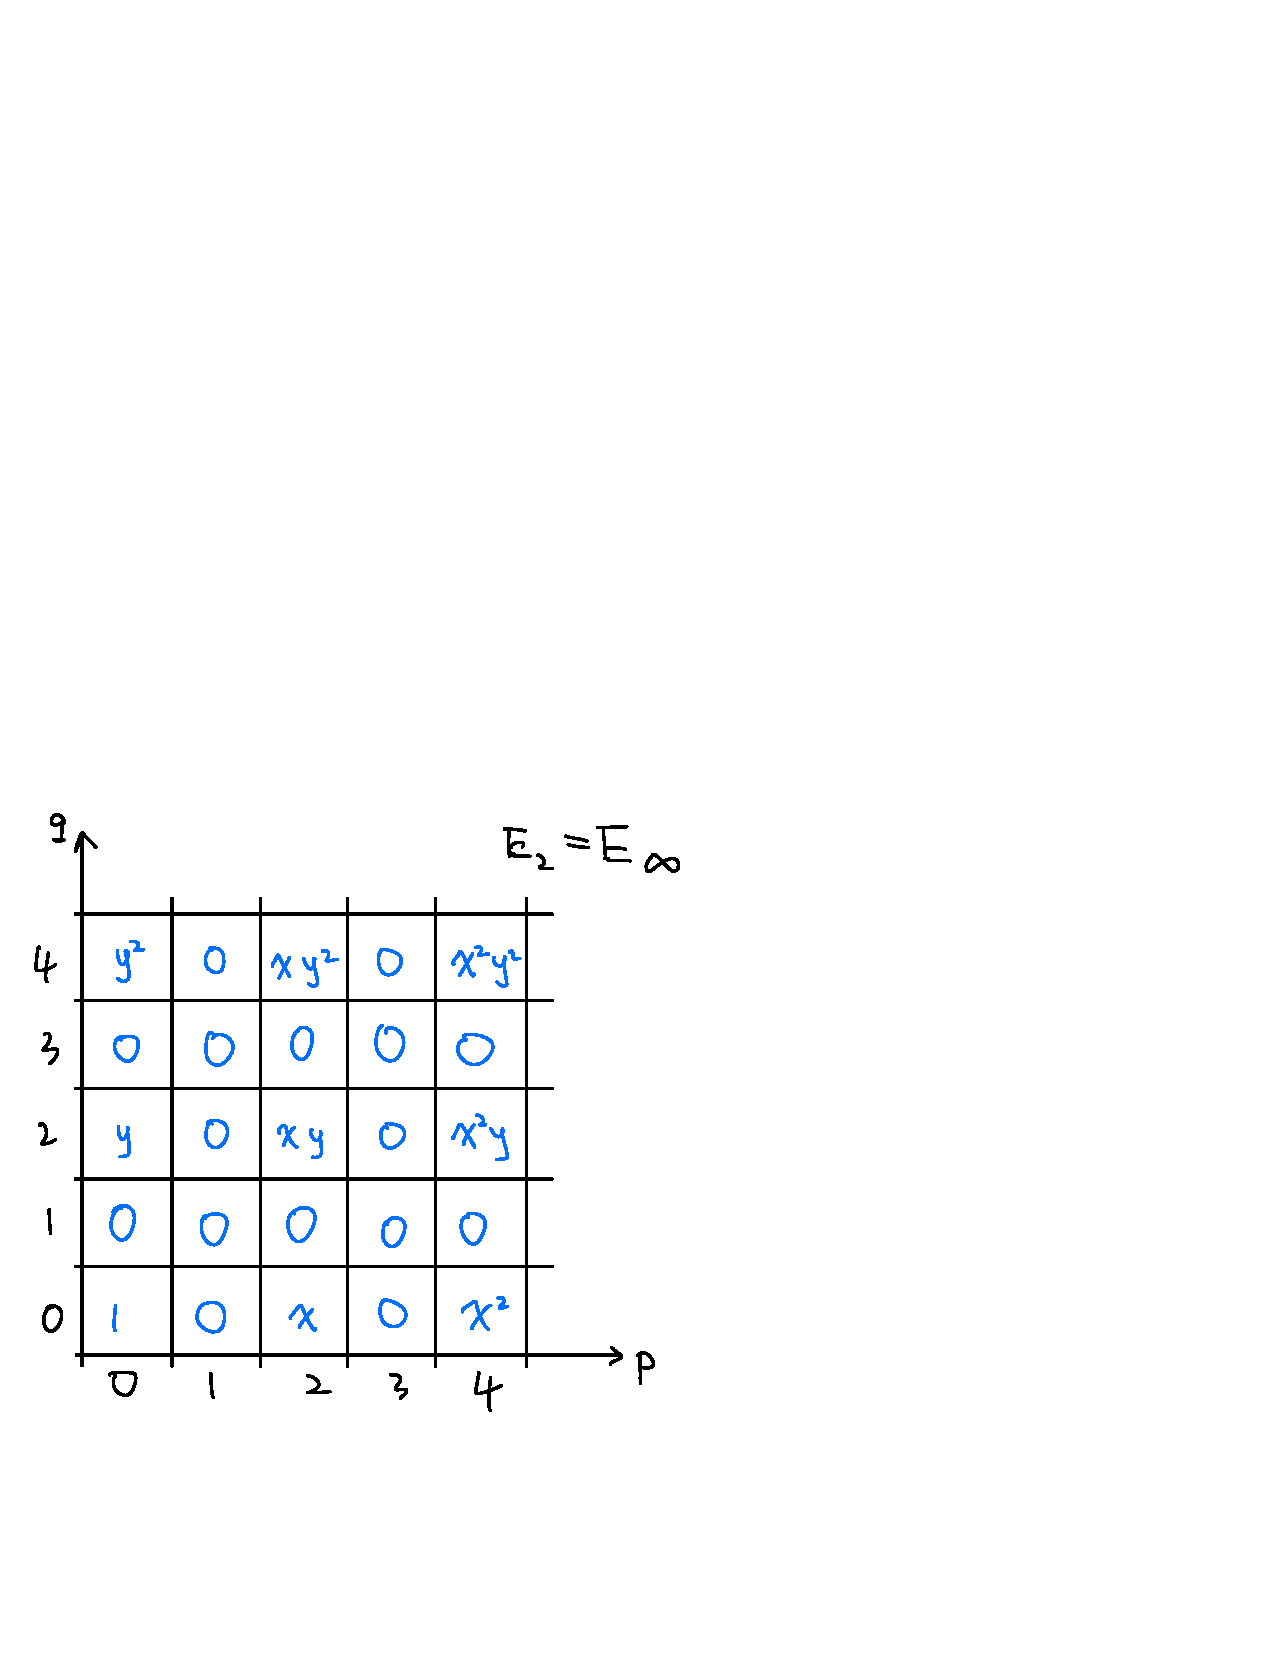
\includegraphics[width=0.5\linewidth]{img/fig12.pdf}
		\caption{$E_2$-page of the LHS spectral sequence of $C_2\to C_4\to C_2$}
		\label{fig:5}
	\end{figure}
	Here every element denotes the generator of $\mathbb{Z}_2$, to see this picture, recall that $|x|=(2,0)$, $|y|=(0,2)$ and $E^2$ is freely generated to obtain all these generators. Obviously, the spectral sequence collapeses at $E_2=E_\infty=\mathbb{Z}[x,y]/(2x,2y)$. But here we encounter the lifting problem. We have two possible algebra structures for $H^\bullet(C_4;\mathbb{Z})$, either $\mathbb{Z}[x,y]/(2x,2y)$ or $\mathbb{Z}[z]/(4z)$. Indeed, the second one is right. Although we do not know the right answer without any other inputs, the solution of the lifting problems here turns out to have only has finite possibilities.
\end{proof}
\begin{remark}
	We emphasize again that using a spectral sequence to compute the (co)homology of $C_4$ is somewhat like {\itshape using a sledgehammer to crack a nut}. As the computation above shows, in order to determine the differentials one typically needs substantial additional information about the (co)homology groups. Although we packaged this input into lemmas, this does not mean that obtaining it is any easier than computing the (co)homology by other methods. Thus, the purpose of this example is purely pedagogical.
\end{remark}

For a less trivial example, and for an illustration of how the associated lifting problems ultimately admit only finitely many solutions, see the disscussion on the dihedral group $D_8$ in \cite[Example 6.4]{ramos2017spectralsequencesexamples}.

However, if we work over $\mathbb{Z}_2$ rather than $\mathbb{Z}$, the lifting problem will disappear. 
\begin{lemma}
	\label{tran}
	Consider an extension of Abelian groups:
	\[
	0\to H\to G\to G/H\to 0
	\]
	We have the following exact sequence:
	\begin{equation}
		\label{five}
		\begin{aligned}
			0\to H^1(G/H;R)\cong &\operatorname{Hom}(G/H,R)\xrightarrow{\mathrm{inf}}H^1(G;R)\cong \operatorname{Hom}(G,R)\\&\xrightarrow{\mathrm{res}}H^1(H,R)\cong\operatorname{Hom}(H,R)\xrightarrow{d_2^{0,1}}H^2(G/H,R)\xrightarrow{\inf}H^2(G,R).
		\end{aligned}
	\end{equation}
	The differential $d^{0,1}_2:E_2^{0,1}\to E_2^{2,0}$ is called {\itshape trangression}.
\end{lemma}
\begin{remark}
	This is a weaker version of \cite[Corollary 7.2.3]{evens1991cohomology}. A similar theorem for Serre spectral sequence can be found in \cite[Theorem 9.13]{davis2001lecture}.
\end{remark}
\begin{example} The $\mathbb{Z}_2$ cohomology ring of $C_4$ is given by:
	\[
	H^\bullet(C_4;\mathbb{Z}_2)=\Lambda(z)\otimes{\mathbb{F}_2[z^{\prime}]},\quad |z|=1,\, |z'|=2
	\]
\end{example}
\begin{proof}
Using the same method we used in the last example, the $E_2$-page looks like Figure~\ref{fig:12}.
\begin{figure}
	\centering
	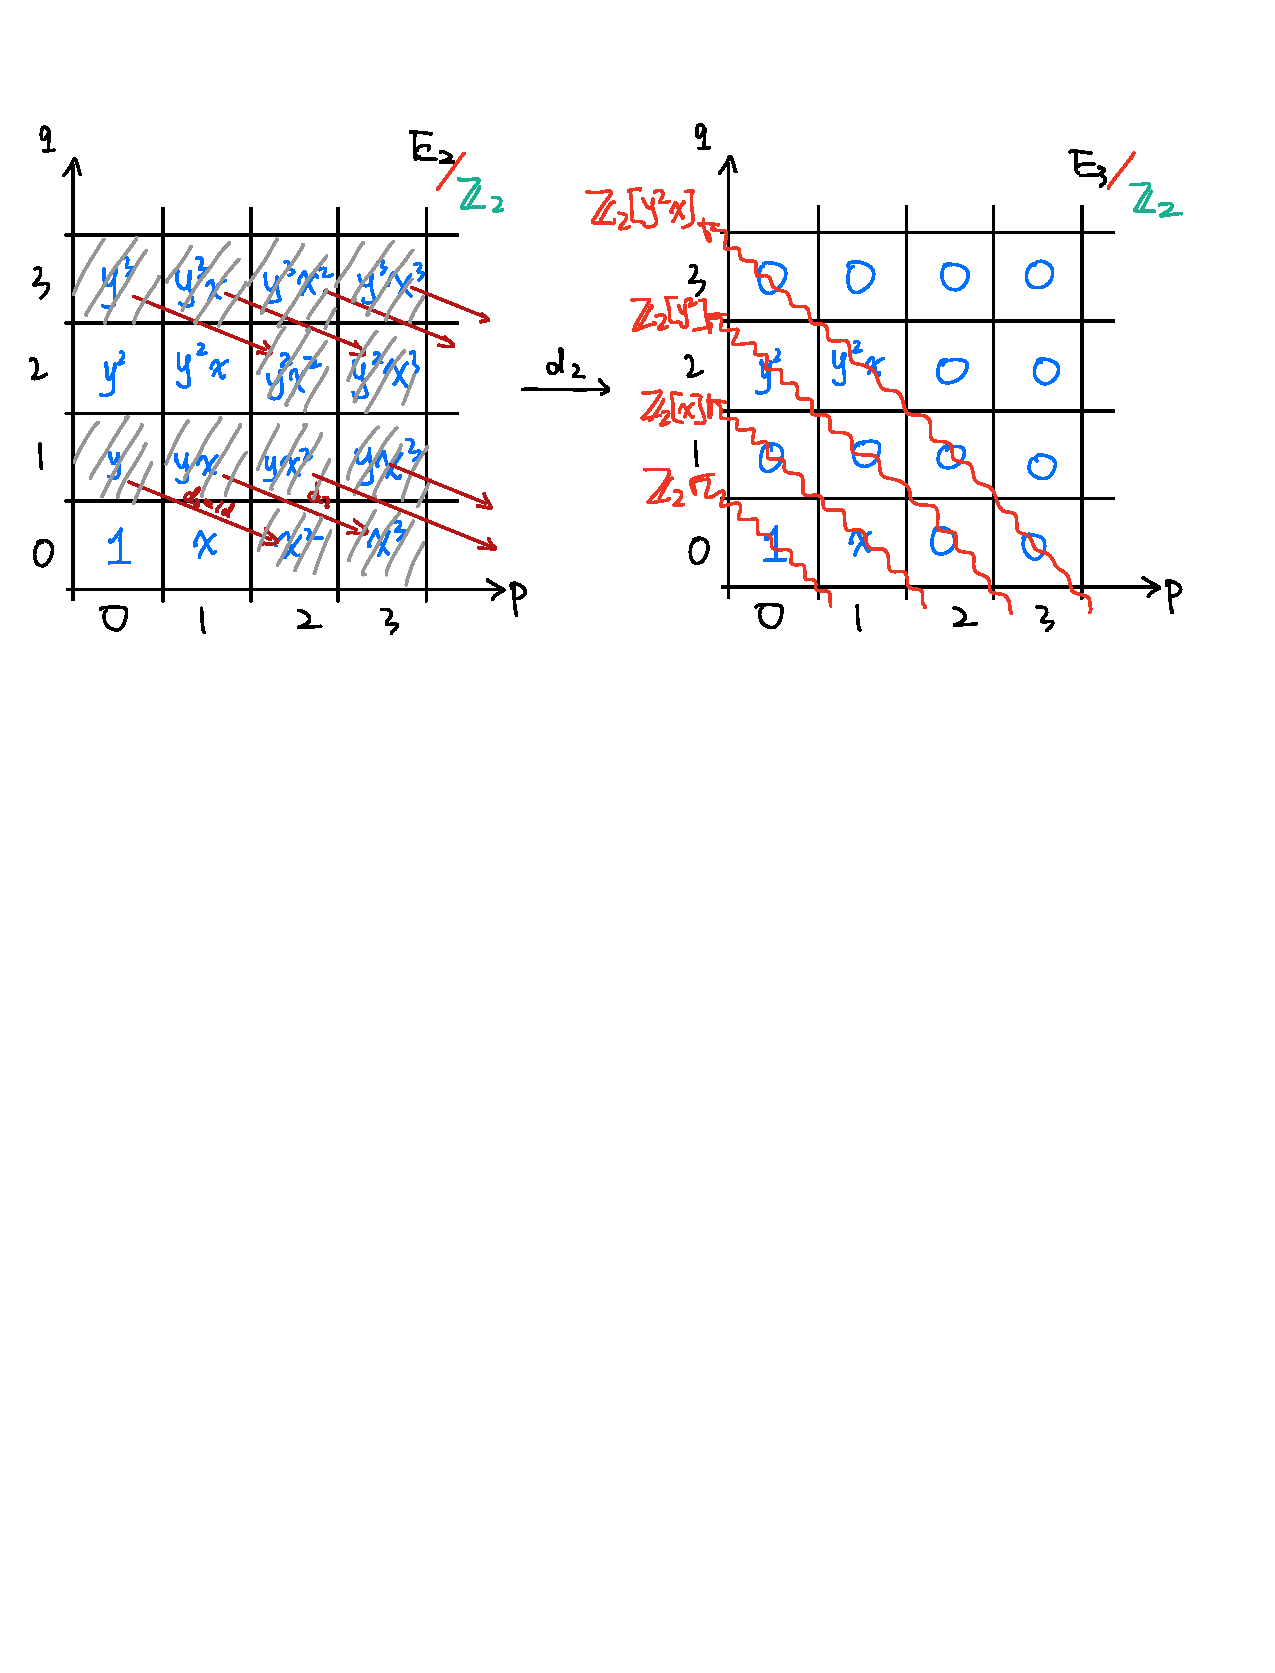
\includegraphics[width=0.8\linewidth]{img/fig13.pdf}
	\caption{$E_2$ and $E_3$-page of LHS spectral sequence of $C_2\to C_4\to C_2$ with $\mathbb{Z}_2$ coefficients.}
	\label{fig:12}
\end{figure}
We need a more careful analysis of $d_2$. Fortunately, Lemma \ref{tran} allows us to determine $d_2^{0,1}$, and the algebra structure then helps us compute the other $d_2^{p,q}$. The five-term exact sequence \cref{five} gives 
\[
\mathrm{Hom}(C_4,\mathbb{Z}_2)\cong\mathbb{Z}_2\xrightarrow{\mathrm{res}}\mathrm{Hom}(C_2,\mathbb{Z}_2)\cong\mathbb{Z}_2\xrightarrow{d^{0,1}_2}H^2(C_4/C_2\cong C_2;\mathbb{Z}_2)
\]
The $[0]_{\mathrm{Hom}}$ in $\mathrm{Hom}(C_4,\mathbb{Z}_2)$ and $\mathrm{Hom}(C_2,\mathbb{Z}_2)$ maps every group elements to $[0]_{\mathbb{Z}_2}$. It's clear that the generator $[1]_{\mathrm{Hom}}$ in $\mathrm{Hom}(C_4,\mathbb{Z}_2)$ maps $\{e,g^2\}$ to $[0]_{\mathbb{Z}_2}$ and maps $\{g,g^3\}$ to $[1]_{\mathbb{Z}_2}$. Similarly,  $[1]_{\mathrm{Hom}}\in\mathrm{Hom}(C_2,\mathbb{Z}_2)$ can be realized by mapping $\{e\}$ to $[0]_{\mathbb{Z}_2}$ and mapping $\{g\}$ to $[1]_{\mathbb{Z}_2}$. If we restrict $C_4$ to $C_2$, then $[1]_{\mathrm{Hom}}\in\mathrm{Hom}(C_4,\mathbb{Z}_2)$ will be mapped to $[0]_{\mathrm{Hom}}\in\mathrm{Hom}(C_2,\mathbb{Z}_2)$. Hence $\mathrm{res}=0$, and $\ker{d^{0,1}_2}=\mathrm{Im}\mathrm{res}=0$. Recall that $d^{0,1}_2: E^{0,1}_2\cong \mathbb{Z}_2\to E^{2,0}_2\cong\mathbb{Z}_2$, so we have only one choice, $d^{0,1}_2=\mathrm{id}$, i.e. $d_2(y)=x^2$.\footnote{We want to point out that if the extension is split, i.e. $C_2\to C_2\times C_2\to C_2$, the $\mathrm{res}$ can be non-zero.}

Next, we can use the Leibniz rule \cref{leib} to determine other $d_2^{p,q}$:
\[
\begin{gathered}
d_2^{1,1}(yx)=d_2(y)x-yd_2(x)=x^3,\quad \text{since~}d_2^{1,0}=0\Rightarrow d_2(x)=0\\
d_2^{p,1}(yx^p)=d_2(y) x^p - y d(x^p)=x^{p+1}
\end{gathered}
\]
Then we conclude that all the $d_2^{p,1}$'s equal $\mathrm{id}$, which means $E^{p\geq 0,1}_2$ and $E^{p\geq 2,0}_2$ will be killed. Following the same argument we can also see that $d_2^{p,3}=\mathrm{id}$, for example:
\[
d^{1,3}_2(y^3x)=d_2(y^3)x-yd_2(x)=d_2(y^3)x= y^2 x^2
\] 
But $d^{p,2}_2$'s are $0$, since:
\[
d_2^{0,2}(y^2)=d_2(y) y - yd_2(y)=x^2y-yx^2 =x^2y-x^2y=0\Rightarrow d_2(y^2x^n)=d_2(y^2) x^n + d_2(x^n)=0
\]
We conclude that $E_3$ looks likes the right panel of Figure~\ref{fig:12}. Obviously, the spectral sequence collapeses at $E_3=E_\infty$. The lifting problem is trivial, we have $H^\bullet(C_4;\mathbb{Z}_2)\cong \mathrm{Tot}(E_
\infty)\cong \Lambda[z=x]\otimes\mathbb{Z}_2[z^{\prime}=y^2]$ with $|z|=1,|z^{\prime}|=2$.
\end{proof}

In this example, we haven't encountered a thorny lifting problem because the $E^\infty$ is a {\itshape  free, graded-commutative, bigraded algebra}, which means the only relation on this algebra is \cref{grad}. Obviously, this is not true for Example \ref{2.12}, where $E_\infty=\mathbb{Z}[x,y]/(2x,2y)$. There, we have two relations $2x=0$ and $2y=0$ to lift. This is the problem. Actually we can conclude: {\itshape If $E_\infty$ is a free, graded-commutative, bigraded algebra, then $H^\bullet$ is a free, graded commutative algebra isomorphic to $\mathrm{Tot}(E_\infty)$.}
\begin{remark}
	$\mathbb{Z}[x,y]/(2x,2y)$ is {\itshape not} equal to $\mathbb{Z}_2[x,y]$, since in the former the constant part is $\mathbb{Z}$, whereas in the latter the constantpart is $\mathbb{Z}_2$. Even though they agree on the nonconstant terms, they are not the same ring. Another subtlety is the following. Consider $|x|=1$, then \cref{grad} tells us $2x^2=0$, but it is {\itshape not} equal to $x^2=0$, since we work on $\mathbb{Z}$ not $\mathbb{Q}$ or $\mathbb{R}$. Then $\mathbb{Z}[x]/(x^2)$ is {\itshape not} free. 
\end{remark}
\subsection{Cellular chain complex revisited}
We can also use spectral sequence directly by finding a nice filtration.
\begin{theorem}
   Let $X$ be a CW complex, then the cellular homology computes the singular homology
   \[
   H_\bullet^{\text{cell}}(X) = H_\bullet (X)
   \]
\end{theorem}
\begin{proof}
Assume that $X$ admits a CW decomposition
\[
X^{(0)}\subset X^{(1)}\subset\cdots\subset X^{(n)}
\]
We define an acending filtration on the singular chain complex $S_\bullet(X)$ by
\[
F_pS(X)=S(X^{(p)})
\]
By \cref{theorem:1.5}, the $E^0$-page is
\[
E_{p,q}^0=\mathrm{Gr}_p(S_{p+q}(X))=\frac{S_{p+q}(X^{(p)})}{S_{p+q}(X^{(p-1)})}=S_{p+q}(X^{(p)},X^{(p-1)})
\]
Therefore the $E^1$-page computes the {\itshape relative homology} \cite[\S2.1]{Hatcher}
\[
E_{p,q}^{1}={H}_{p+q}(X^{(p)},X^{(p-1)})=\begin{cases}C_{p}^{\text{cell}}(X),&q=0\\0,&q\neq0\end{cases}
\]
which is the definition of cellular chains. To compute $E^2$-page, we need to know $d_1: C^{\text{cell}}_p(X)\to C^{\text{cell}}_{p-1}(X)$. If it coincidents with the differential in cellular homology, then we have 
\[
E_{p,q}^{2}=\begin{cases}H_{p}^{\text{cell}}(X),&q=0\\0,&q\neq0\end{cases}
\]
It is clear that the spectral sequence collapses at $E^2=E^\infty$. Hence we prove that cellular homology is equivalent to singular homology. We now explain why this is indeed the case.

Recall that \eqref{eq:2} tells us $d_1$ is induced by the boxed part of the following chain, where we chose $r=1$, $q=0$
\begin{equation}
	S_{p+1}(X^{(p+1)})\to \boxed{
	S_{p}(X^{(p)})\xrightarrow{d}S_{p-1}(X^{(p-1)})
	}\to S_{p-2}(X^{(p-2)})
\end{equation}
Then we need to induce $d_1: H_p(X^{(p)},X^{(p-1)})\to H_{p-1}(X^{(p-1)},X^{(p-2)})$ from $d$. To do that, note that $d(S_p(X^{p-1}))\subset S_{p-1}(X^{p-1})$, then we have an induced map:
\[
d_\# :S_p(X^{(p)},X^{(p-1)})\to S_{p-1}(X^{(p-1)})
\]
Togather with $j_\#$ induced from including $j:X^{(p-1)}\to (X^{(p-1)},X^{(p-2)})$
\[
S_p(X^{(p)},X^{(p-1)})\xrightarrow{d_\#}S_{p-1}(X^{(p-1)})\xrightarrow{j_\#} S_{p-1}(X^{(p-1)},X^{(p-2)})
\]
then $d_1$ is induced by applying the homology functor:
\[
d_1:H_p(X^{(p)},X^{(p-1)})\xrightarrow{d_*}H_{p-1}(X^{(p-1)})\xrightarrow{j_*} H_{p-1}(X^{(p-1)},X^{(p-2)})
\]
$d_*$ is exactly the definition of $\partial_*$ in the following long exact sequence \cite[\S2 注记 1.4]{jiang}\footnote{Sorry, I cited a Chinese book here, because I could not find a presentation in other references that I found satisfactory.}
\[
\cdots\overset{\partial_*}{\operatorname*{\operatorname*{\longrightarrow}}}H_q(X^{(p-1)})\overset{i_*}{\operatorname*{\operatorname*{\longrightarrow}}}H_q(X^{(p)})\overset{j_*}{\operatorname*{\operatorname*{\longrightarrow}}}H_q(X^{(p)},X^{(p-1)})\overset{\partial_*}{\operatorname*{\operatorname*{\longrightarrow}}}H_{q-1}(X^{(p-1)})\overset{i_*}{\operatorname*{\operatorname*{\longrightarrow}}}\cdots
\]
induced by the short exact sequence of singular chain complex \cite[\S 定理 1.11]{jiang}\footnote{\cite{jiang} works on general relative cellular homology. One can recover the setting of our discussion by taking the minimal space to be the empty set.}
\[
0\longrightarrow S_*(X^{(p-1)})\xrightarrow{i_\#}S_*(X^{(p)})\xrightarrow{j_\#}S_*(X^{(p)},X^{(p-1)})\longrightarrow0
\]
However the definition of the diffrential in cellular homology is exactly $j_*\circ \partial_*$. \cite[\S3 命题2.3]{jiang} Hence we complete the proof.
\end{proof}

\section{AH spectral sequence and K-theoretic classification of D-branes}
\label{sec:AHSS}
Consider a spacetime of the form $\mathbb{R}\times X_9$, where $X_9$ is a nine-dimensional (possibly non-compact) space. We study Type II A/B string theory on this background. It is well known that string theory contains non-perturbative degrees of freedom called $D$-branes. A $D$-brane can wrap a cycle in $X_9$, and it couples to Ramond–Ramond (RR) fields, hence it can carry RR charge. A natural question is: how should one classify the charges of $D$-branes?

A naive expectation is that, since the RR charge is a gauge charge, it should take values in the de Rham cohomology $H^{\mathrm{DR}}(X_9;\mathbb{R})$, imposing Dirac quantization would then suggest that it should in fact lie in the integral cohomology $H(X_9;\mathbb{Z})$. However, explicit computations of RR charges carried by $D$-branes in \cite{Green:1996dd,Minasian:1997mm} show that ordinary cohomology is not sufficient to capture all information about $D$-brane charge, and that a more appropriate mathematical framework is $K$-theory.

One physical motivation is that open strings can end on $D$-branes. From the viewpoint of the low-energy effective theory on the brane worldvolume, a stack of $N$ coincident $D$-branes gives rise to a $U(N)$ gauge theory. Equivalently, a $D$-brane configuration is not merely a cycle in $X_9$: it naturally comes equipped with a vector bundle. Ordinary cohomology is too coarse to encode such bundle data, whereas $K$-theory is designed precisely to classify vector bundles. In this sense, cohomological classification fails to distinguish certain $D$-brane configurations that are physically inequivalent. In \cite{Witten:1998cd}, Witten provided a physical explanation for the $K$-theoretic classification of $D$-brane charge using brane–antibrane annihilation in the framwork of the Sen’s tachyon condensation conjecture \cite{Sen:1998sm}.

In this report, we adopt an interpretive framework slightly different from Witten’s, while building on his work. Following \cite{Maldacena:2001xj,Moore:2003vf}, we relate the physical consistency conditions on possible $D$-brane configurations to computations in the AH spectral sequence, thereby explaining why $D$-brane charges should be classified by $K$-theory rather than by ordinary cohomology.

Here, we consider a more general case in which there is a cohomological nontrivial $H$-field. We ask what cycles $\mathcal{W}\subset X_9$ can be wrapped by a D-brane, and whether such configurations are stable. An unstable D-brane configuration is equivalent to vacuum, so we need to {\itshape modulo} it out. If D-branes were classified by original cohomology, then free branes can wrap any homologically nontrivial cycle in $X_9$ anda a brane wrapping a nontrivial cycle is absolutely stabe. 

However, the field theory on the D-brane must be consistent. It can be shown \cite{Freed:1999vc,Kapustin:1999di} that a D-brane must wrap $\mathcal{W}\subset{X}_9$ which satisfies:
\begin{equation}
	\label{A}
	W_3(\mathcal{W})+\left.[H]\right|_{\mathcal{W}}=0,\quad\text{~in~}H^3(\mathcal{W};\mathbb{Z})
\end{equation}
to be anomaly free. Here $W_3(\mathcal{W})$ is the {\itshape integral  Stiefel-Whitney class} (\cref{bock}) of $T\mathcal{W}$.  Suppose there is a cycle $\mathcal{W}'\subset X_9$ on which:
\[
W_3(\mathcal{W}‘)+\left.[H]\right|_{\mathcal{W}’}\neq0
\]
According to \eqref{A}, we cannot wrap a D-brane on $\mathcal{W}'$. Let us do so anyway, with an unstable D-brane {\itshape instanton}, i.e. one wrapping on a spatial cycle. As we have just explained, a D-brane instanton is not anomaly free, but we can cancel the anomalies by adding a new brane wrapped on the spatial cycle $\mathcal{W}\subset \mathcal{W}'$ and propagates in time. By Poincar\'e duality (PD), this new D-brane ending on $\mathcal{W}$  provides a magnetic source such that:
\begin{equation}
	\label{B}
	\operatorname{PD}(\mathcal{W}\subset\mathcal{W}')=W_3(\mathcal{W}')+\left.[H]\right|_{\mathcal{W}'}
\end{equation}
Indeed, it really does cancel the anomalies. We refer the reader to \cite{Freed:2000ta} for details. Hence the physical picture is that a $D$-brane wrapping the spatial cycle $\mathcal{W}$ propagates for some time and then ends on a $D$-brane instanton wrapping $\mathcal{W}'$, as illustrated in Figure~\ref{fig:11}. 

\begin{figure}
	\centering
	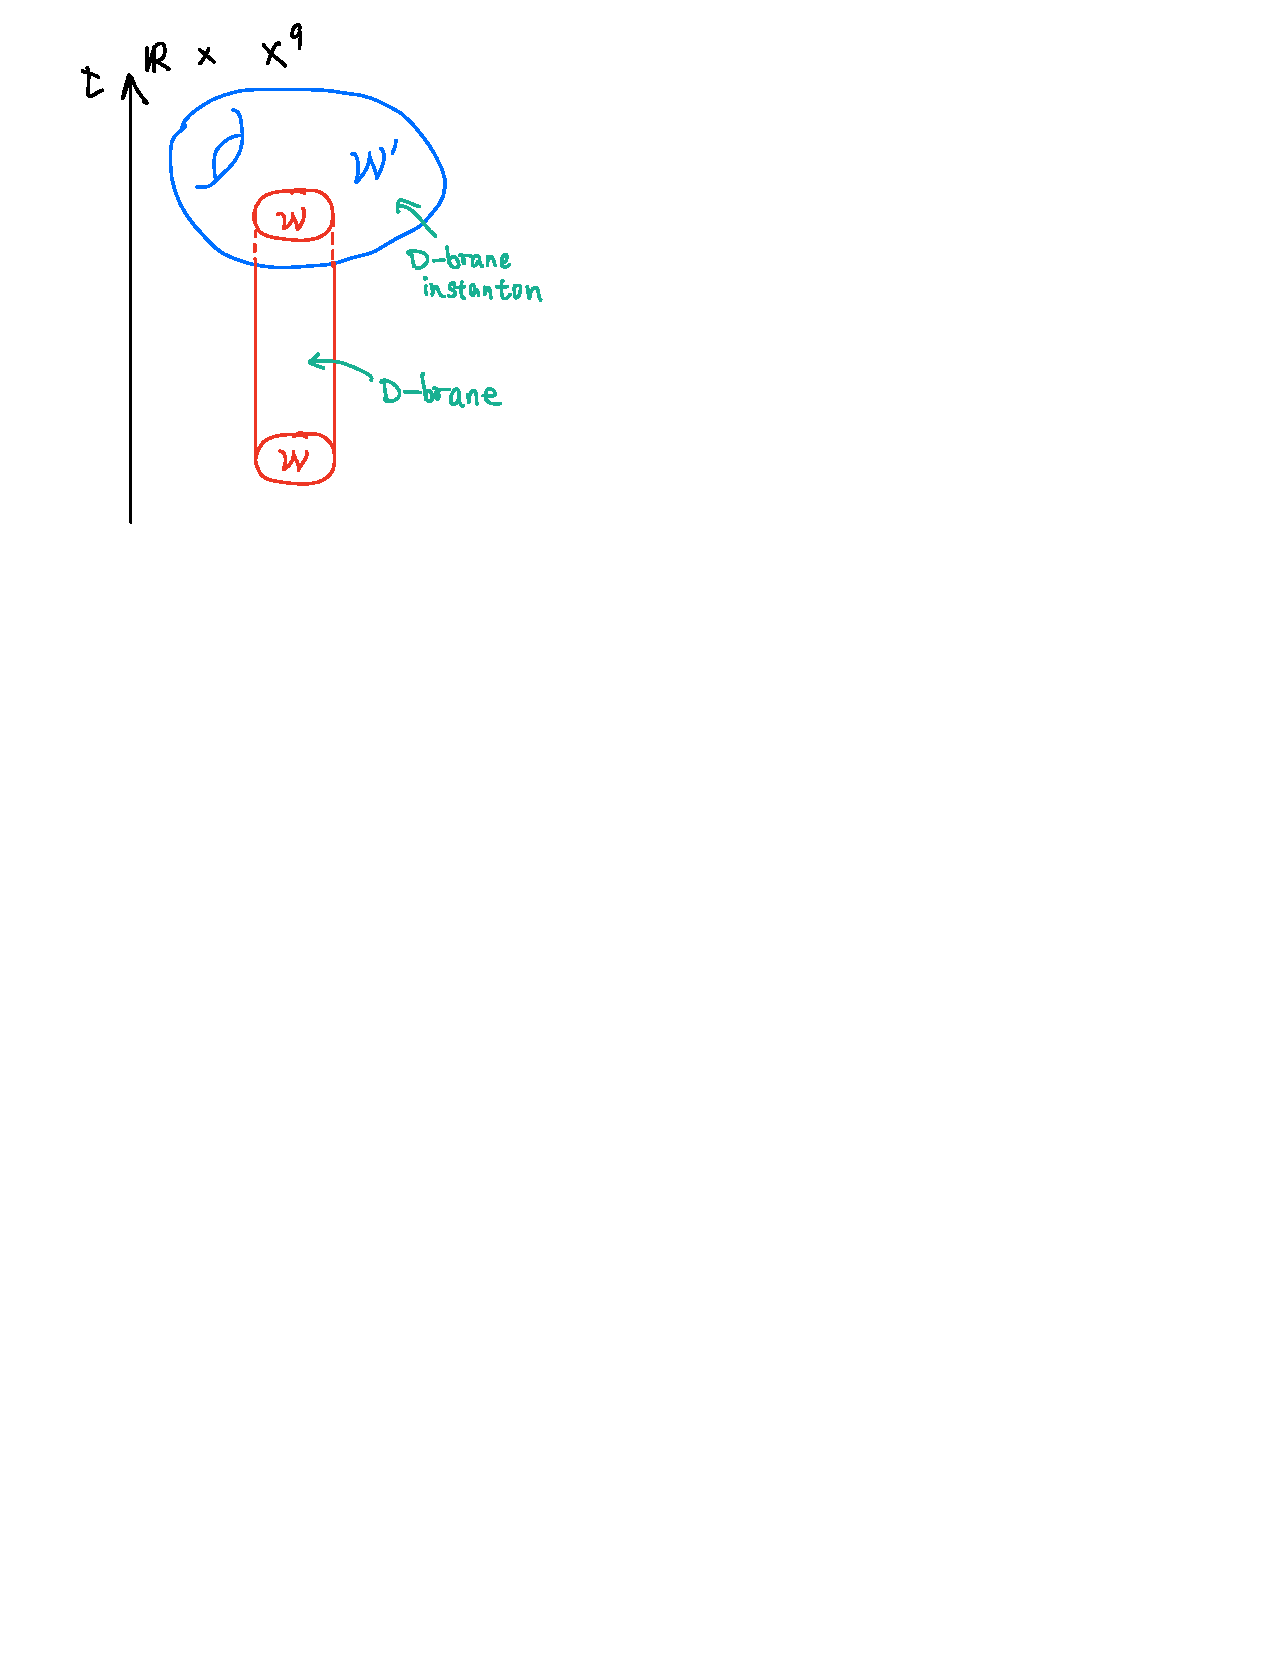
\includegraphics[width=0.4\linewidth]{img/fig14.pdf}
	\caption{$D$-brane/$D$-brane-instanton system}
	\label{fig:11}
\end{figure}

From the discussion around \eqref{B}, we know that this $D$-brane/$D$-brane-instanton system is anomaly-free in the sense of \eqref{A}, and therefore it can be regarded as an allowed $D$-brane configuration. However, due to the presence of the $D$-brane instanton, the system quickly decays to the vacuum and is thus unstable. We will see later that this is analogous to the fact that a D-brane is the differential of a D-brane instanton, so it is exact and should be modded out. In summary, $D$-brane charges should be classified by the quotient $\eqref{A}/\eqref{B}$. In the presence of a cohomologically nontrivial $H$-field, the relevant mathematical framework is {\itshape twisted $K$-theory} denoted by $K^\bullet_H$. We will not go into the mathematical details here. The interested reader may consult \cite{Atiyah:2004jv}.

We now analyze more carefully what \eqref{A} and \eqref{B} mean mathematically. Note that our discussion here is largely qualitative. A complete quantitative dictionary does not seem likely to exist. Nevertheless, it is sufficient to provide a clear picture of how these physical conclusions are tied to the $K$-theoretic classification of $D$-branes.

Consider the trivial fibration $*\hookrightarrow X_9\twoheadrightarrow X_9$ introduced in \cref{CP} for computing $K^\bullet({\mathbb{C}P^{n}})$. From the $E_2$-page, it is clear that ordinary integral cohomology is the {\itshape first approximation} of $K$-theory:
\[
\begin{aligned}
&K^0(X_9)\sim E_2^{\mathrm{even}}(X_9):=\oplus_{j\mathrm{~even}}H^j(X_9;\mathbf{Z})\\
&K^1(X_9)\sim E_2^{\mathrm{odd}}(X_9):=\oplus_{j\mathrm{~odd}}H^j(X_9;\mathbf{Z})
\end{aligned}
\]
The first nonzero differential is $d_3$. In ordinary $K$-theory it was identified in \cite{atiyah1961vector} as $d_3=\operatorname{Sq}^3_{\mathbb{Z}}$ and generalized for twisted $K$-theory as $d_3^H=\operatorname{Sq}^3_{\mathbb{Z}}+H\smile$ in \cite{rosenberg1982homological}. These formulae were rediscovered in a physics context \cite{Diaconescu:2000wy} later. Here $\operatorname{Sq}^3_{\mathbb{Z}}$ is the {\itshape integral Steenrod operator} (\cref{SA}). Now, let us "prove" \footnote{A careful reader may notice that, in the following chain of formulas, the cup products of cohomology classes are taken between elements that live in different cohomology rings, which seems wrong. In fact, this is only because we have been a bit careless and suppressed some inclusion maps and canonical isomorphisms that physicists find annoying. This level of rigor is sufficient for physicists, but I’m sure it won’t escape Lean’s scrutiny.
} a relationship between $H(E_2,d_3)$ and the physical conditions \eqref{A} and \eqref{B}.

First we want to look closely at $\ker d_3$, and we need the following formula: \cite[\S 8]{milnor1974characteristic}
\begin{equation}
	\label{eq:thom}
	Sq^i(\tau_{\mathcal{W}\in X_9})=T^*(w_i(\mathcal{W}))\sim w_i\smile \tau_{\mathcal{W}\in X_9}
\end{equation}
Where $\tau_{\mathcal{W}\in X_9}$ denotes the{ \itshape{Thom class}} (\cref{Thom}) of $\mathcal{W}\in X_9$, and $\sim$ is justified by \eqref{Tiso}, with the pullback suppressed, so we use $\sim$ instead of $=$. In perticular, consider $i=2$ and denote $a\in H^{\bullet}(X_9)$ by $\operatorname{PD}_{X_9}(a)=\mathcal{W}$. From the definition of the Thom class, we know that $a=\tau_{\mathcal{W}\subset X_9}$. Recall that the definition of the Integral Stiefel-Whitney class and Integral Steenrod operator comes from Bockstein homomorphism (\cref{bock}). Then we have $Sq^3\approx W_3\smile$ which implies:
\[
\large d_3(a)=0\quad\Leftrightarrow\quad\left(W_3(\mathcal{W})+[H]\right)\smile a=0
\]
Next, let us interpret the quotient by $\operatorname{Im}d_3$, suppose $a=d_3(a')$. Then use PD
\[
\operatorname{PD}(a)=\mathcal{W},\quad \operatorname{PD}(a')=\mathcal{W}'
\]
use the definition of the Thom class like we did before, we know that $a=\tau_{\mathcal{W}\subset X_9}$ and $a'=\tau_{\mathcal{W}'\subset X_9}$. We pause here to prove a lemma first.

\begin{lemma}
	\label{poor}
	Consider $A\overset{i}{\hookrightarrow}B\overset{j}{\hookrightarrow}C$, where $A$ is of codimension $k$ in $B$ and $B$ is of codimension $l$ in $C$. We have:
	\[
	\tau_{A\subset B}\smile \tau_{B\subset C}=\tau_{A\subset C}
	\]
\end{lemma}
\begin{proof}
From \eqref{thomiso} and \eqref{nature}, one can easily show that the following diagram commutes:
\[
\begin{tikzcd}
	{H^{q+k}(B,B-A)} && {H^{q+k+l}(C,C-B)} \\
	& {H^{q+k}(B)} \\
	{H^{q}(A)} && {H^{q+k+l}(C)} \\
	& {H^{q+k+l}(C,C-A)}
	\arrow[color=blue,"{\iota^*}", from=1-1, to=2-2]
	\arrow[color=blue,"{\iota^*}", from=1-3, to=3-3]
	\arrow[color=blue,"{T^*}","\cong"', from=2-2, to=1-3]
	\arrow["{j^!}", from=2-2, to=3-3]
	\arrow[color=blue,"{T^*}","\cong"', from=3-1, to=1-1]
	\arrow["{i^!}", from=3-1, to=2-2]
	\arrow["{(i\circ j)^!}"', from=3-1, to=3-3]
	\arrow[color=red,"{T^*}"',"\cong", from=3-1, to=4-2]
	\arrow[color=red,"{\iota^*}"', from=4-2, to=3-3]
\end{tikzcd}
\]
 Consider $[1]_A\in H^0(A)$ and follow its image in $H^{k+l}(C)$. Along the blue arrows, it first maps to $\tau_{A\subset B}\sim \tau_{A\subset B}\smile[1]_B$ and then is sent to $\tau_{A\subset B}\smile \tau_{B\subset C}$. We can also follow the red arrows, in which case the answer is $\tau_{A\subset C}$. The commutativity of the diagram tells us that they are equl. 
\end{proof}
Now we can prove that condition \eqref{B} implies that one should take the quotient by $\operatorname{Im}d_3$.
\begin{theorem}
	\[
	\operatorname{PD}\left(\mathcal{W}\subset\mathcal{W}^{\prime}\right)=W_3(\mathcal{W}^{\prime})+[H]|_{\mathcal{W}^{\prime}}\quad\Rightarrow\quad a=d_3(a^{\prime})
	\]
\end{theorem}
\begin{proof}
	As we explained before, $\mathrm{rhs}\smile a' =d_3(a')$. In terms of the Thom class formulation, what we need to prove is that
	\[
	\operatorname{PD}_{\mathcal{W}'}(\mathcal{W})\smile \tau_{\mathcal{W}'\subset X_9} =\tau_{\mathcal{W}\subset{X}_9}
	\]
	Note that $	\operatorname{PD}_{\mathcal{W}'}(\mathcal{W})=\tau_{\mathcal{W}\subset\mathcal{W}'}$, using Lemma \ref{poor} we complete the proof.
\end{proof}
Up to this point, we can see that the physical outcome \eqref{A} modulo \eqref{B} has a mathematical counterpart in the AH spectral sequence computation of $K$-theory. Namely, it corresponds to the {\itshape second approximation} to $K^\bullet$ obtained after taking the $d_3$-differential. In this sense, one seems to obtain a physical explanation of the $K$-theoretic classification of D-branes.

It must be emphasized, however, that we have hidden many subtle drawbacks.
First, we have only discussed the differential $d_3$. The higher differentials $d_r$ are already difficult to describe mathematically, and it is even harder to relate them to physics. Second, even if all differentials $d_r$ were known, the stabilized $E_\infty$-page still gives only an approximation to $K^\bullet$, because it determines only the associated graded group $\operatorname{G}(K^\bullet)$ rather than $K^\bullet$ itself. On the other hand, the heuristic "proofs'' above indicate that the condition $\eqref{A}/\eqref{B}$ is actually stronger than $\ker(d_3)/\operatorname{Im}(d_3)$. This extra strength might compensate, at least partially, for the two approximations mentioned above.
Anyway, the argument here provides strong support for the viewpoint that starting from the two physical requirements on D-branes, the resulting computation leads to $K$-theory.

In \cite{Maldacena:2001xj,Moore:2003vf} this idea was used to compute the twisted $K$-theory of $SU(3)$ from physical considerations, and \cite{Braun:2003rd, Rosenberg:2017iej} extended the computation to other compact simple Lie groups.

\appendix
\section{Some basic notions from algebraic topology}
In this appendix, we collect several basic concepts used in the main text for completeness. These materials can be found in standard algebraic topology textbooks, and some of them are briefly reviewed in Tachikawa-san’s lecture notes. Here we only supplement a few important definitions and formulas that will be used in the main text. Topics that are already treated in detail in Tachikawa-san’s notes, such as Stiefel--Whitney classes, will not be repeated here.

\subsection{Steenrod algebra}
\label{SA}
We can describe Steenrod operators by the following axiomatic defination:
\begin{definition}
	For each $i \geq 0$, there exists a {\itshape cohomology operation} (i.e. a natural transfermation between to cohomology functors) $Sq^i:H^n(-,\mathbb{Z}_2)\to H^{n+i}(-,\mathbb{Z}_2)$, such that:
	\begin{enumerate}
		\item $Sq^0=\mathrm{id}$
		\item $Sq^1$ is the Bockstein homomorphism $\beta$ associated with the sequence $0\to \mathbb{Z}_2\to \mathbb{Z}_4\to \mathbb{Z}_2\to0$ . 
		\item $Sq^{i}=0$ for $i>n$ and $Sq^{i=n}(x)= x\smile x$
		\item $Sq^i(f^*(\alpha))=f^*(Sq^i(\alpha))$ for $f:X\to Y$
		\item $Sq^i(\alpha+\beta)=Sq^i(\alpha)+Sq^i(\beta)$
		\item (Cartan formula): \[Sq^k(a\smile b)=\sum_{i+j=k}Sq^i(a)\smile Sq^j(b)\]
		\item (Adam relations): for $i$ even\[Sq^i\circ Sq^j=\sum_{k=0}^{i/2}\binom{j-k-1}{i-2k}Sq^{i+j-k}\circ Sq^k\]
		\item $Sq^i$ is stable under suspension, i.e. $Sq^i(\sigma(\alpha))=\sigma(Sq^i(\alpha))$ where $\sigma:H^n(X;\mathbb{Z}_2)\to H^{n+1}(\Sigma X;\mathbb{Z}_2)$
	\end{enumerate}
\end{definition}
The last condition is very useful in homotopy theory. The explicit construction of Steenrod operators can be found in \cite[\S 2]{mosher2008cohomology}. Since we can compose the $Sq^i$'s, Steenrod squares become an algebra. Moreover, the Cartan formula tells us it also has a {\itshape coproduct}. In fact Steenrod algebra is a {\itshape Hopf algebra}.
\subsection{Thom isomorphism theorem}
The Thom isomorphism theorem can be stated for a complex pair, in this report, one just chooses $A=\emptyset$.
\label{Thom}
\begin{theorem}[Thom isomorphism theorem]\label{thm:thom-iso}
	Let $(M,A)$ be an oriented relative manifold of dimension $n+k$.
	Let $N\supset A$ be a submanifold of $M$ such that $(N,A)$ is an oriented relative manifold of dimension $n$.
	Then there exists an isomorphism
	$$
	T^*\colon H^q(N- A)\longrightarrow H^{q+k}(M- A,\,M- N),
	$$
	called the Thom isomorphism.
	The image of the unit $[1]\in H^0(N\setminus A)$ under $T^*$,
	$$
	\tau:=T^*([1])\in H^k(M- A,\,M- N),
	$$
	is called the Thom class of $N- A$ in $M-A$.
	Let $j\colon N- A\hookrightarrow M-A$ denote the inclusion.
	Then, for any $\xi\in H^q(M-A)$,
	\begin{equation}
		\label{Tiso}
		T^*(j^*\xi)=\xi\smile\tau.
	\end{equation}
	Here $\smile$ denotes the cup product
	$$
	\smile\colon H^q(M-A)\times H^k(M- A,\,M- N)\longrightarrow H^{q+k}(M-A,\,M- N).
	$$
\end{theorem}
There is a corollary \cite[\S 5 推论 7.2]{jiang} from the Thom isomorphism theorem, the following diagram commutes:
\begin{equation}
	\label{thomiso}
	\begin{tikzcd}
		{H^q(N)} & {H^{q+k}(M,M-N)} \\
		& {H^{q+k}(M)}
		\arrow["{T^*}","\cong"', from=1-1, to=1-2]
		\arrow["{h^!}"', from=1-1, to=2-2]
		\arrow["{\iota^*}", from=1-2, to=2-2]
	\end{tikzcd}
\end{equation}
where the {\itshape transfer homomorphism} is defined by,
$$
\begin{tikzcd}
	H_*(M) \arrow[r, "f_*"] & H_*(N) \\
	H^{m-*}(M)
	\arrow[u, "\operatorname{PD}_M"' , "\cong"]
	\arrow[r, "f^!"] &
	H^{n-*}(N)
	\arrow[u, "\operatorname{PD}_N"' , "\cong"]
\end{tikzcd}
\qquad\qquad
\begin{tikzcd}
	H^*(M) \arrow[d, "\operatorname{PD}_M"', "\cong"] & 
	H^*(N) \arrow[l, "f^*"'] \arrow[d, "\operatorname{PD}_N"', "\cong"] \\
	H_{m-*}(M) &
	H_{n-*}(N) \arrow[l, "f_!"']
\end{tikzcd}
$$
from $(f\circ g)_*=f_*\circ g_*$, it is clear that
\begin{equation}
	\label{nature}
	(f\circ g)^!=f^!\circ g^!
\end{equation}
A simplified way to say this is: \cref{thomiso} tells us that the Thom class of the submanifold (a cohomology class) and its orientation class (a homology class) are Poincar\'e dual to each other in the ambient manifold. This fact is used repeatedly throughout this report.

In \cref{eq:thom}, we introduce the relationship between the Stiefel--Whitney class and the Steenrod operator. Here is a generalized statement.
\begin{theorem}[Thom--Wu, \cite{adams1992formulae}]
	Let $M$ be a compact differentiable $n$-manifold, not necessarily orientable, with fundamental class
	$[M]\in H_n(M;\mathbb{Z}_2)$. Then there is a unique class $v_i\in H^i(M;\mathbb{Z}_2)$, called the Wu class such that
	\[
	\langle Sq^i (x),\,[M]\rangle=\langle v_i\smile x,\,[M]\rangle
	\]
	for each $x\in H^{n-i}(M;\mathbb{Z}_2)$, and the Stiefel--Whitney classes $w_k\in H^k(M;\mathbb{Z}_2)$
	satisfy
	\[
	w_k=\sum_{i+j=k} Sq^j (v_i).
	\]
\end{theorem}
For example, the second Wu class satisfies $v_2=w_1^2+w_2$ and for an orientable manifold $w_1=0$.
\subsection{Bockstein homomorphism}
\label{bock}
If we apply the covariant functor $\mathrm{Hom}(C_n(X),-)$ on a short exact sequence of abelian groups $0\boldsymbol{\to}G\boldsymbol{\to}H\boldsymbol{\to}K\boldsymbol{\to}0$. we obtain a short exat sequence of chain complexes,
\[
0\to C^n(X;G)\to C^n(X;H)\to C^n(X;K)\to0
\]
which induces a long exact sequence of cohomology groups,
\[
\cdots\to H^n(X;G)\to H^n(X;H)\to H^n(X;K)\overset{\beta}{\to} H^{n+1}(X;G)\to\cdots
\]
The boundary map $\beta$ is called the {\itshape Bockstein homomorphism}. We are interested in the following extension:
\[
0\to\mathbb{Z}\xrightarrow{\times 2}\mathbb{Z}\xrightarrow{\mathrm{mod}\,2}\mathbb{Z}_2\to0
\]
which induces $\beta: H^n(X;\mathbb{Z}_2)\to H^{n+1}(X;\mathbb{Z})$. The original Stiefel--Whitney class and Steenrod operator are defined over $\mathbb{Z}_2$. Now we can define their integral counterparts by:
\[
W_3:=\beta(w_3),\quad Sq^3_{\mathbb{Z}}:=\beta\circ Sq^2\circ r
\]
where $r$ means reducing $H^n(X;\mathbb{Z})$ to $H^{n}(X;\mathbb{Z}_2)$.
\acknowledgments
We thank ChatGPT for help with English polishing. All mathematical and physical content in this report was prepared by me based on the cited literature; any theorems and definitions stated here come from papers or textbooks rather than from conversations with ChatGPT. B. Zheng would like to thank Y. Chen for helpful disscusion.

\paragraph{Note added.} Although this term-end report is primarily a survey, some of the arguments do not have direct counterparts in the literature, and parts of the discussion reflect the author’s own views. Readers should therefore read it critically. In particular, in \cref{sec:AHSS}, I did not fully understand some of the proofs, and the relevant material is included mainly as a pointer to the literature for the reader’s reference. Moreover, I cannot guarantee that the proofs included here are the most concise, or even correct at all, since they are written from the perspective of a physics student with a rather shallow understanding of mathematics, not a professional mathematician.

\bibliographystyle{JHEP}
\bibliography{refs}

\end{document}
